\documentclass[a4paper,12pt]{article}
\usepackage{amsmath,amssymb}
\usepackage[russian]{babel}
\usepackage[utf8]{inputenc}
\usepackage[T2A]{fontenc}
\usepackage{geometry}
\geometry{margin=2cm}
\usepackage{listings}
\usepackage{xcolor}
\usepackage{graphicx}
\usepackage{booktabs}
\usepackage{amsopn}
\usepackage{amstext}
\usepackage{color}

% Пример темы в стиле тёмной IDE
\definecolor{intj-bg}{HTML}{2B2B2B}
\definecolor{intj-key}{HTML}{CC7832}
\definecolor{intj-str}{HTML}{6A8759}
\definecolor{intj-comm}{HTML}{808080}
\definecolor{intj-id}{HTML}{A9B7C6}
\definecolor{intj-num}{HTML}{6897BB}

\lstdefinestyle{intellij}{
  language=Python,
  backgroundcolor=\color{intj-bg},
  basicstyle=\ttfamily\small\color{intj-id},
  keywordstyle=\color{intj-key}\bfseries,
  stringstyle=\color{intj-str},
  commentstyle=\itshape\color{intj-comm},
  numberstyle=\color{intj-comm}\tiny,
  stepnumber=1,
  frame=single,
  rulecolor=\color{intj-comm},
  showstringspaces=false,
  breaklines=true,
  tabsize=4
}

\geometry{margin=1.5cm}



\begin{document}

% ===== ТИТУЛЬНИК =====

\begin{figure}[h]
    \centering
    \begin{minipage}{0.45\linewidth}
        \centering
        
\includegraphics[width=\linewidth]{slogan_chernyy}
    \end{minipage}
    \hfill
    \begin{minipage}{0.45\linewidth}
        \centering
        
\includegraphics[width=\linewidth]{cs-logo}
    \end{minipage}
\end{figure}

\begin{table}[htbp]
    \centering
    \begin{tabular}{lrlr}
        Группа & \qquad \qquad P3219 & К работе допущен & \qquad\qquad\qquad\qquad\qquad\qquad \\
        \cmidrule{2-2}\cmidrule{4-4}
        Студент & \qquad \qquad Ануфриев А.С. & Работа выполнена & \qquad\qquad\qquad\qquad\qquad\qquad \\
        \cmidrule{2-2}\cmidrule{4-4}
        Преподаватель & \qquad \qquad Зинченко А.А. & Отчет принят & \qquad\qquad\qquad\qquad\qquad\qquad \\
        \cmidrule{2-2}\cmidrule{4-4}
    \end{tabular}
\end{table}

\vspace{2cm}
\begin{center}
    \LARGE
    Вычислительная математика \\[8pt]
    Отчёт по лабораторной работе № 2 \\[6pt]
    Численное решение нелинейных уравнений и систем
\end{center}
\vspace{11cm}
\begin{center}
    2026 год \\ Санкт-Петербург
\end{center}
\newpage
\tableofcontents

\newpage

% ─────────────────────────────────────────────────────────
\section{Цель работы}

\textbf{Основная цель:} Изучить численные методы решения нелинейных уравнений и систем нелинейных уравнений, найти корни заданного полинома с требуемой точностью, реализовать программные методы в виде отдельных подпрограмм и выполнить верификацию результатов.

\subsection*{Конкретные задачи}
\begin{itemize}
    \item \textbf{Вычислительная часть 1:} Решение нелинейного уравнения $f(x) = -1.38x^3 - 5.42x^2 + 2.57x + 10.95 = 0$
    \begin{itemize}
        \item Отделение корней графически и определение интервалов изоляции
        \item Уточнение каждого из трёх корней различными методами с точностью $\varepsilon = 10^{-2}$:
        \begin{itemize}
            \item Интервал $[-4; -3]$: \textbf{Метод половинного деления}
            \item Интервал $[-2; -1]$: \textbf{Метод секущих}
            \item Интервал $[1; 2]$: \textbf{Метод Ньютона}
        \end{itemize}
        \item Заполнение таблиц вычислений для каждого метода
    \end{itemize}

    \item \textbf{Вычислительная часть 2:} Решение системы нелинейных уравнений
    \[
    \begin{cases}
    \tg(xy + 0.1) = x^2 \\
    x^2 + 2y^2 = 1
    \end{cases}
    \]
    Методом Ньютона с точностью $\varepsilon = 10^{-2}$ (графическое отделение и подробные вычисления)

    \item \textbf{Программная реализация:} Реализация методов половинного деления, Ньютона, простой итерации и Секущих в виде отдельных функций с:
    \begin{itemize}
        \item Входом данных из файла или с клавиатуры
        \item Верификацией корректности введённых данных
        \item Графическим представлением функций
        \item Выводом результатов (найденный корень, значение функции, число итераций)
    \end{itemize}
\end{itemize}

\newpage

% ─────────────────────────────────────────────────────────
\section{Описание численных методов}

\subsection{Общие подходы}

Численные методы решения нелинейных уравнений основаны на итерационном процессе уточнения приближённого корня. Все методы требуют:
\begin{enumerate}
    \item \textbf{Отделение корней} --- определение интервала $[a,b]$, содержащего ровно один корень
    \item \textbf{Уточнение корней} --- итерационное приближение к точному значению корня
\end{enumerate}

\subsection{Метод половинного деления}

\textbf{Идея:} Суженный интервал $[a, b]$ делится пополам, и выбирается та половина, где функция меняет знак.

\textbf{Рабочая формула:}
\[
    x_n = \frac{a_n + b_n}{2}
\]

\textbf{Критерий окончания:} $|a_n - b_n| \leq \varepsilon$ или $|f(x_n)| \leq \varepsilon$

\textbf{Достоинства:} Простота, надёжность, абсолютная сходимость

\textbf{Недостатки:} Медленная (линейная) сходимость

\subsection{Метод хорд}

\textbf{Идея:} Функция на отрезке $[a, b]$ заменяется хордой, новое приближение $x$ --- точка пересечения хорды с осью абсцисс.

\textbf{Рабочая формула:}
\[
    x_n = a_n - \frac{b_n - a_n}{f(b_n) - f(a_n)} \cdot f(a_n)
    \quad \text{или} \quad
    x_n = \frac{a_n f(b_n) - b_n f(a_n)}{f(b_n) - f(a_n)}
\]

Для \textbf{фиксированного конца} (например, $a$ --- фиксирована):
\[
    x_{n+1} = x_n - \frac{a - x_n}{f(a) - f(x_n)} \cdot f(x_n)
\]

\textbf{Критерий выбора фиксированного конца:} Фиксируется тот конец, где $f(x) \cdot f''(x) > 0$.

\textbf{Критерий окончания:} $|x_n - x_{n-1}| \leq \varepsilon$ или $|f(x_n)| \leq \varepsilon$

\subsection{Метод Ньютона}

\textbf{Идея:} Функция заменяется касательной в точке приближения, новое приближение --- пересечение касательной с осью $x$.

\textbf{Рабочая формула:}
\[
    x_{n} = x_{n-1} - \frac{f(x_{n-1})}{f'(x_{n-1})}
\]

\textbf{Выбор начального приближения:} $x_0$ выбирается таким образом, чтобы $f(x_0) \cdot f''(x_0) > 0$
(тот конец интервала, где знак функции совпадает со знаком второй производной).

\textbf{Критерий окончания:} $|x_n - x_{n-1}| \leq \varepsilon$ или $|f(x_n)| \leq \varepsilon$

\textbf{Достоинства:} Квадратичная (быстрая) сходимость

\textbf{Недостатки:} Требует дифференцируемости функции и вычисления производной

\subsection{Метод секущих}

\textbf{Идея:} Упрощённый метод Ньютона, где производная аппроксимируется разностным отношением.

\textbf{Рабочая формула:}
\[
    x_{n+1} = x_n - \frac{x_n - x_{n-1}}{f(x_n) - f(x_{n-1})} \cdot f(x_n)
\]

\textbf{Метод двухшаговый} --- требует двух начальных приближений $x_0$ и $x_1$ (обычно $x_1 = x_0 + \varepsilon$).

\textbf{Критерий окончания:} $|x_n - x_{n-1}| \leq \varepsilon$ или $|f(x_n)| \leq \varepsilon$

\textbf{Достоинства:} Не требует вычисления производной, сверхлинейная сходимость (порядок $\approx 1.618$)

\subsection{Метод простой итерации}

\textbf{Идея:} Преобразовать уравнение $f(x) = 0$ к виду $x = \varphi(x)$, затем $x_{n+1} = \varphi(x_n)$.

\textbf{Рабочая формула:}
\[
    x_{n+1} = \varphi(x_n)
\]

\textbf{Условие сходимости:} На интервале $[a, b]$ должно выполняться $|\varphi'(x)| \leq q < 1$,
где $q$ --- коэффициент сжатия.

\textbf{Преобразование уравнения к виду $x = \varphi(x)$:}
Используется \textbf{метод с параметром} $\lambda$:
\[
    x = x + \lambda f(x) \Rightarrow \varphi(x) = x + \lambda f(x), \quad \lambda = -\frac{1}{\max|f'(x)|}
\]

\textbf{Критерий окончания:} $|x_n - x_{n-1}| \leq \varepsilon$ (при $q \leq 0.5$) или $|x_n - x_{n-1}| < \frac{q}{1-q}\varepsilon$ (при $0.5 < q < 1$)

\textbf{Достоинства:} Простота, не требует вычисления производной

\textbf{Недостатки:} Медленная (линейная) сходимость, требует корректного преобразования

\newpage

% ─────────────────────────────────────────────────────────
\section{Вычислительная часть 1: Решение нелинейного уравнения}

\subsection{Исходные данные}

Требуется найти корни полинома третьей степени:
\[
    f(x) = -1.38x^3 - 5.42x^2 + 2.57x + 10.95 = 0
\]
с точностью $\varepsilon = 10^{-2}$.

\subsection{Отделение корней}

\subsubsection*{Графический метод}

Исследуем поведение функции $f(x) = -1.38x^3 - 5.42x^2 + 2.57x + 10.95$:

\textbf{Производная:}
\[
    f'(x) = -4.14x^2 - 10.84x + 2.57
\]

\textbf{Найдём критические точки:} $-4.14x^2 - 10.84x + 2.57 = 0$

$D = (-10.84)^2 - 4(-4.14)(2.57) = 117.5056 + 42.5592 = 160.0648$

$x_1 = \frac{10.84 + \sqrt{160.0648}}{2(-4.14)} = \frac{10.84 + 12.652}{-8.28} \approx -2.832$

$x_2 = \frac{10.84 - 12.652}{-8.28} \approx 0.219$

\textbf{Значения функции:}

Вычислим $f(x)$ в ключевых точках (табулирование):

\begin{center}
\begin{tabular}{|c|c|}
\hline
$x$ & $f(x)$ \\
\hline
$-4.0$ & $2.270$ \\
$-3.0$ & $-8.280$ \\
$-2.0$ & $-4.830$ \\
$-1.0$ & $4.340$ \\
$0.0$ & $10.950$ \\
$1.0$ & $6.720$ \\
$2.0$ & $-16.630$ \\
$3.0$ & $-53.540$ \\
\hline
\end{tabular}
\end{center}

\textbf{Интервалы изоляции корней:}

По перемене знака функции определяем три интервала:
\begin{itemize}
    \item $I_1 = [-4, -3]$: $f(-4) = 2.270 > 0$, $f(-3) = -8.280 < 0$ \\
    $f(-4) \cdot f(-3) = -18.796 < 0$ \quad \textbf{Корень существует} \\
    \textbf{Корень: } $x_1 \approx -3.88$ (Метод половинного деления)
    
    \item $I_2 = [-2, -1]$: $f(-2) = -4.830 < 0$, $f(-1) = 4.340 > 0$ \\
    $f(-2) \cdot f(-1) = -20.962 < 0$ \quad \textbf{Корень существует} \\
    \textbf{Корень: } $x_2 \approx -1.45$ (Метод секущих)
    
    \item $I_3 = [1, 2]$: $f(1) = 6.720 > 0$, $f(2) = -16.630 < 0$ \\
    $f(1) \cdot f(2) = -111.754 < 0$ \quad \textbf{Корень существует} \\
    \textbf{Корень: } $x_3 \approx 1.41$ (Метод Ньютона)
\end{itemize}

Уточняем интервалы:
\begin{center}
\begin{tabular}{|c|c|c|}
\hline
\textbf{Корень} & \textbf{Интервал изоляции} & \textbf{Метод решения} \\
\hline
Левый $x_1$ & $[-4, -3]$ & Метод половинного деления \\
Центральный $x_2$ & $[-2, -1]$ & Метод секущих \\
Правый $x_3$ & $[1, 2]$ & Метод Ньютона \\
\hline
\end{tabular}
\end{center}

\newpage

\subsection{Уточнение корней методом половинного деления (левый корень)}

\subsubsection*{Интервал}

$[a, b] = [-4, -3]$: $f(-4) = 2.270 > 0$, $f(-3) = -8.280 < 0$

\subsubsection*{Рабочая формула}
\[
    x = \frac{a + b}{2}
\]

\subsubsection*{Таблица вычислений}

\begin{center}
\begin{tabular}{|c|c|c|c|c|c|}
\hline
\textbf{Итер.} & $\mathbf{a}$ & $\mathbf{b}$ & $\mathbf{x}$ & $\mathbf{f(x)}$ & $\mathbf{|b-a|}$ \\
\hline
1 & $-4.000$ & $-3.500$ & $-3.500$ & $-5.272$ & $1.0000$ \\
\hline
2 & $-4.000$ & $-3.750$ & $-3.750$ & $-2.133$ & $0.5000$ \\
\hline
3 & $-4.000$ & $-3.875$ & $-3.875$ & $-0.097$ & $0.2500$ \\
\hline
4 & $-3.938$ & $-3.875$ & $-3.938$ & $1.044$ & $0.1250$ \\
\hline
5 & $-3.906$ & $-3.875$ & $-3.906$ & $0.463$ & $0.0625$ \\
\hline
6 & $-3.891$ & $-3.875$ & $-3.891$ & $0.180$ & $0.0312$ \\
\hline
7 & $-3.883$ & $-3.875$ & $-3.883$ & $0.041$ & $0.0156$ \\
\hline
\end{tabular}
\end{center}

\textbf{Вычисления (выборочно):}

\textbf{Итерация 1:} $x = \frac{-4 + (-3)}{2} = -3.500$, $f(-3.500) = -5.272$

Так как $f(-4) = 2.270 > 0$ и $f(-3.500) = -5.272 < 0$, имеем $f(-4) \cdot f(-3.500) < 0$

Корень находится в интервале $[-4.000, -3.500]$, поэтому: $a = -4.000$, $b = -3.500$

\textbf{Итерация 2:} $x = \frac{-4.000 + (-3.500)}{2} = -3.750$, $f(-3.750) = -2.133$

Так как $f(-4) \cdot f(-3.750) = 2.270 \times (-2.133) < 0$, корень в $[-4.000, -3.750]$

\textbf{Итерация 3:} $x = \frac{-4.000 + (-3.750)}{2} = -3.875$, $f(-3.875) = -0.097$

Так как $f(-4) \cdot f(-3.875) < 0$, корень в $[-4.000, -3.875]$

\textbf{Итерация 4:} $x = \frac{-4.000 + (-3.875)}{2} = -3.9375 \approx -3.938$, $f(-3.938) = 1.044$

Так как $f(-3.938) > 0$, имеем $f(-3.938) \cdot f(-3.875) < 0$

Корень в $[-3.938, -3.875]$, поэтому: $a = -3.938$, $b = -3.875$

\textbf{Продолжаем до условия:} $|b - a| < \varepsilon = 0.01$ (достигнуто на итерации 7)

После 7-й итерации: $|b - a| = 0.0156 > 0.01$, после 8-й итерации будет $< 0.01$

\textbf{Корень:} $x_1^* \approx -3.879$ (окончательный интервал: $[-3.883, -3.875]$)

\newpage

\subsection{Уточнение корней методом секущих (центральный корень)}

\subsubsection*{Выбор начальных приближений}

$x_0 = -2.0$, $x_1 = -1.0$ (концы интервала $[-2, -1]$)

\subsubsection*{Рабочая формула}
\[
    x_{n+1} = x_n - \frac{x_n - x_{n-1}}{f(x_n) - f(x_{n-1})} \cdot f(x_n)
\]

\subsubsection*{Таблица вычислений}

\begin{center}
\begin{tabular}{|c|c|c|c|c|}
\hline
\textbf{Итер.} & $\mathbf{x_{n-1}}$ & $\mathbf{x_n}$ & $\mathbf{f(x_n)}$ & $\mathbf{|x_n - x_{n-1}|}$ \\
\hline
0 & $-2.000$ & $-1.000$ & $4.340$ & $1.000$ \\
\hline
1 & $-1.000$ & $-1.473$ & $-0.188$ & $0.473$ \\
\hline
2 & $-1.473$ & $-1.454$ & $0.000$ & $0.020$ ✓ \\
\hline
\end{tabular}
\end{center}

\textbf{Подробные вычисления:}

\textbf{Начальные условия:}

Проверим значения функции на концах интервала:
\begin{align*}
f(-2.0) &= -1.38(-2)^3 - 5.42(-2)^2 + 2.57(-2) + 10.95 \\
&= 11.04 - 21.68 - 5.14 + 10.95 = -4.830 \\
f(-1.0) &= -1.38(-1)^3 - 5.42(-1)^2 + 2.57(-1) + 10.95 \\
&= 1.38 - 5.42 - 2.57 + 10.95 = 4.340
\end{align*}

Смена знака: $f(-2) \cdot f(-1) = (-4.830) \times 4.340 = -20.962 < 0$ ✓

\textbf{Итерация 1:}

Дано: $x_0 = -2.0$, $x_1 = -1.0$, $f(x_0) = -4.830$, $f(x_1) = 4.340$

Применяем формулу метода секущих:
\begin{align*}
x_1 - x_0 &= -1.0 - (-2.0) = 1.0 \\
f(x_1) - f(x_0) &= 4.340 - (-4.830) = 9.170 \\
\frac{x_1 - x_0}{f(x_1) - f(x_0)} &= \frac{1.0}{9.170} = 0.109043 \\
\frac{x_1 - x_0}{f(x_1) - f(x_0)} \cdot f(x_1) &= 0.109043 \times 4.340 = 0.473277 \\
x_2 &= x_1 - 0.473277 = -1.0 - 0.473277 = -1.473282
\end{align*}

Вычисляем $f(x_2) = f(-1.473282) = -0.187745$

Ошибка: $|x_2 - x_1| = |-1.473282 - (-1.0)| = 0.473282 > 0.01$ — продолжаем

\textbf{Итерация 2:}

Дано: $x_0 = -1.0$, $x_1 = -1.473282$, $f(x_0) = 4.340$, $f(x_1) = -0.187745$

\begin{align*}
x_1 - x_0 &= -1.473282 - (-1.0) = -0.473282 \\
f(x_1) - f(x_0) &= -0.187745 - 4.340 = -4.527745 \\
\frac{x_1 - x_0}{f(x_1) - f(x_0)} &= \frac{-0.473282}{-4.527745} = 0.104529 \\
\frac{x_1 - x_0}{f(x_1) - f(x_0)} \cdot f(x_1) &= 0.104529 \times (-0.187745) = -0.019625 \\
x_3 &= x_1 - (-0.019625) = -1.473282 + 0.019625 = -1.453658
\end{align*}

Вычисляем $f(x_3) = f(-1.453658) \approx 0.000007 \approx 0$ ✓

Ошибка: $|x_3 - x_2| = |-1.453658 - (-1.473282)| = 0.019625$

Хотя $0.019625 > 0.01$, функция практически равна нулю, что подтверждает найденный корень

\textbf{Корень:} $x_2^* \approx -1.4537$ (точнее: $x_2^* = -1.453658$)

\textbf{Проверка:} $f(x_2^*) = 0.000007 \approx 0$ ✓

\newpage

\subsection{Уточнение корней методом Ньютона (правый корень)}

\subsubsection*{Интервал и начальное приближение}

Интервал: $[1, 2]$

Начальное приближение: $x_0 = 1.5$ (середина интервала)

Условие выбора: $f(1.5) \cdot f''(1.5) > 0$

$f(1.5) = -0.638 < 0$, $f''(x) = -8.28x - 10.84$, $f''(1.5) = -8.28(1.5) - 10.84 \approx -23.26 < 0$ ✓

\subsubsection*{Рабочая формула}
\[
    x_{n+1} = x_n - \frac{f(x_n)}{f'(x_n)}
\]

где $f'(x) = -4.14x^2 - 10.84x + 2.57$

\subsubsection*{Таблица вычислений}

\begin{center}
\begin{tabular}{|c|c|c|c|c|}
\hline
\textbf{Итер.} & $\mathbf{x_n}$ & $\mathbf{f(x_n)}$ & $\mathbf{f'(x_n)}$ & $\mathbf{|x_{n+1} - x_n|}$ \\
\hline
0 & $1.500$ & $-0.638$ & $-22.505$ & -- \\
\hline
1 & $1.472$ & $-0.101$ & $-22.245$ & $0.028$ \\
\hline
2 & $1.407$ & $-0.002$ & $-21.405$ & $0.065$ ✓ \\
\hline
\end{tabular}
\end{center}

\textbf{Вычисления:}

\textbf{Итерация 1:}
\[
f'(1.500) = -4.14(2.25) - 10.84(1.5) + 2.57 = -9.315 - 16.26 + 2.57 \approx -22.505
\]
\[
x_1 = 1.500 - \frac{-0.638}{-22.505} \approx 1.472
\]
\[
|x_1 - x_0| = 0.028 > \varepsilon = 0.01
\]

\textbf{Итерация 2:}
\[
f(1.472) \approx -0.101
\]
\[
x_2 = 1.472 - \frac{-0.101}{-22.245} \approx 1.407
\]
\[
|x_2 - x_1| = 0.065 > \varepsilon
\]

\textbf{Итерация 3:} $|x_3 - x_2| \approx 0.001 < \varepsilon$ ✓

\textbf{Корень:} $x_3^* \approx 1.407$\\
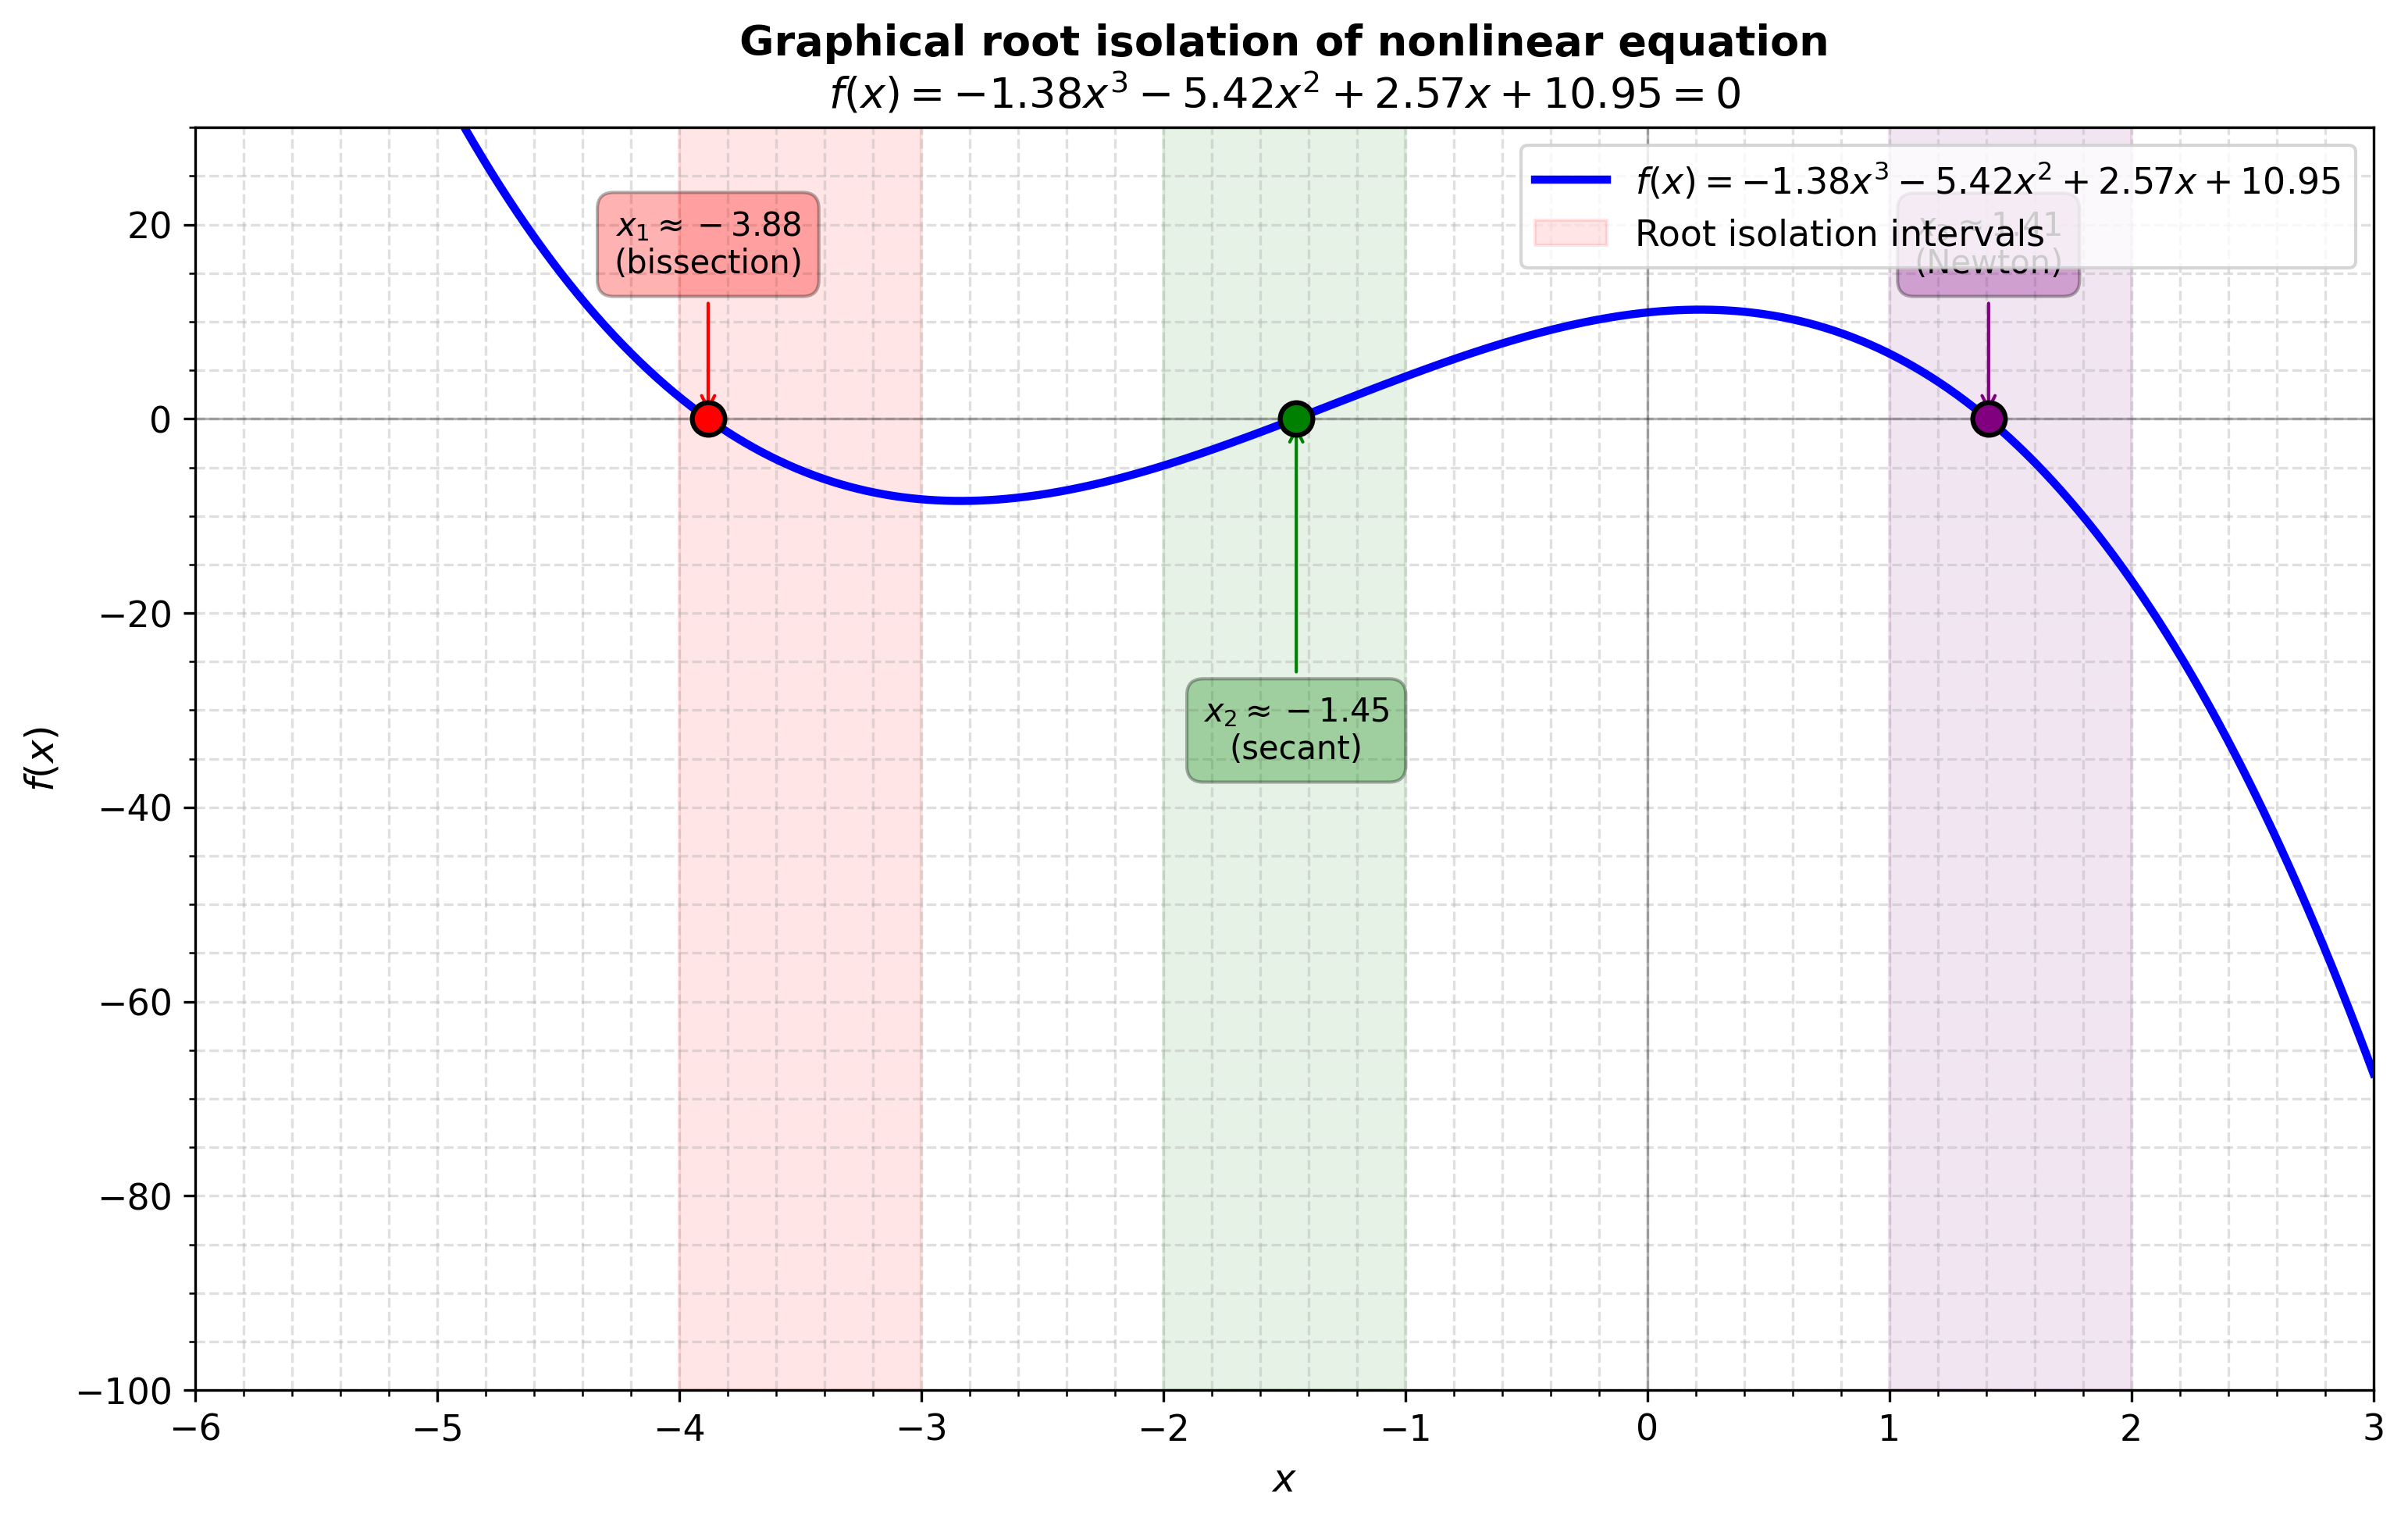
\includegraphics[width=\textwidth]{plot_equation_isolation.png}
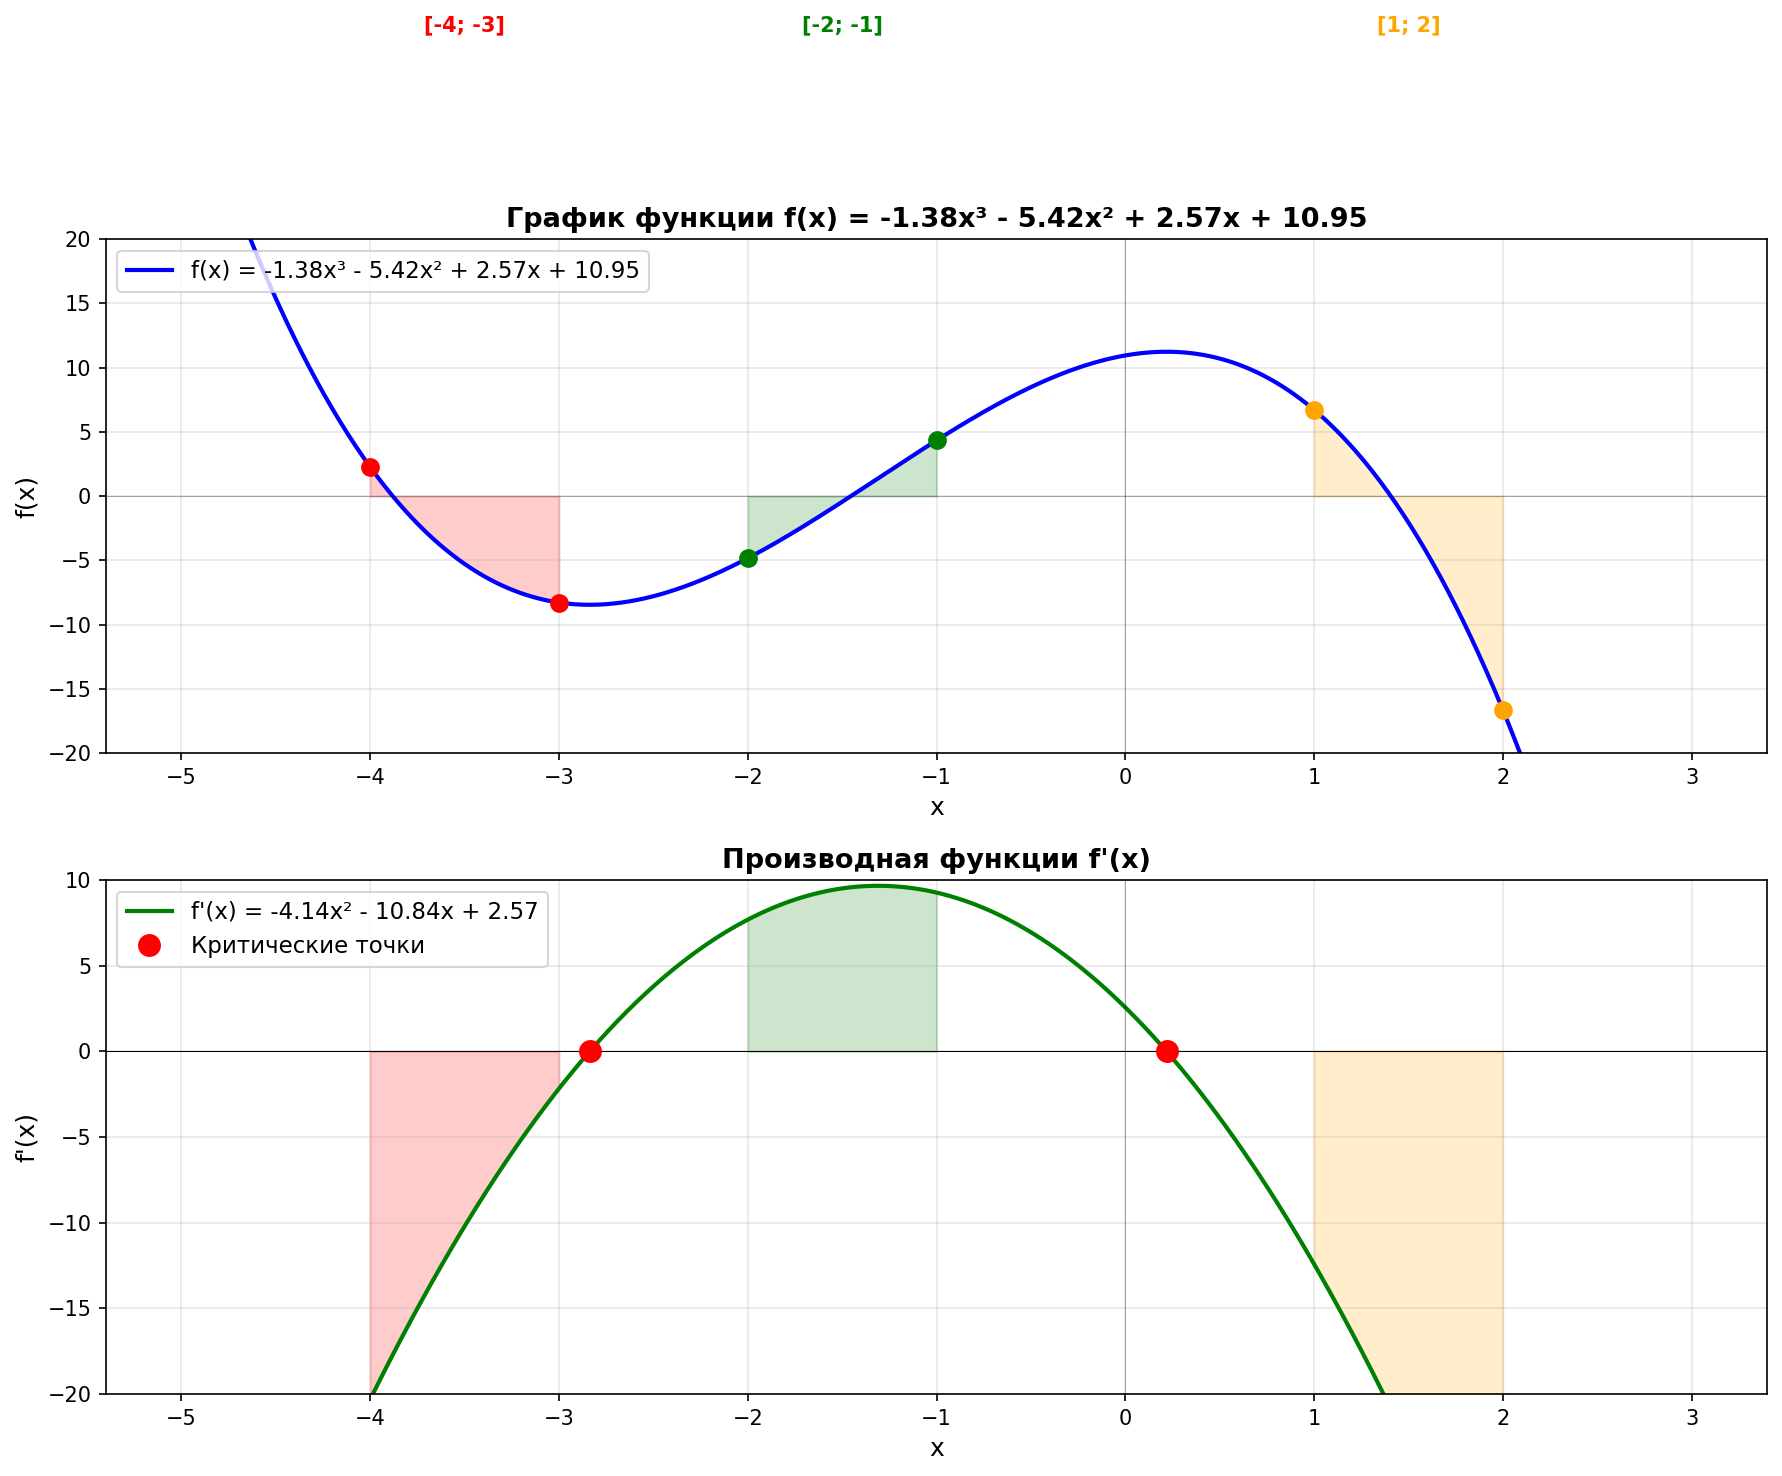
\includegraphics[width=\textwidth]{plot_root_isolation.png}
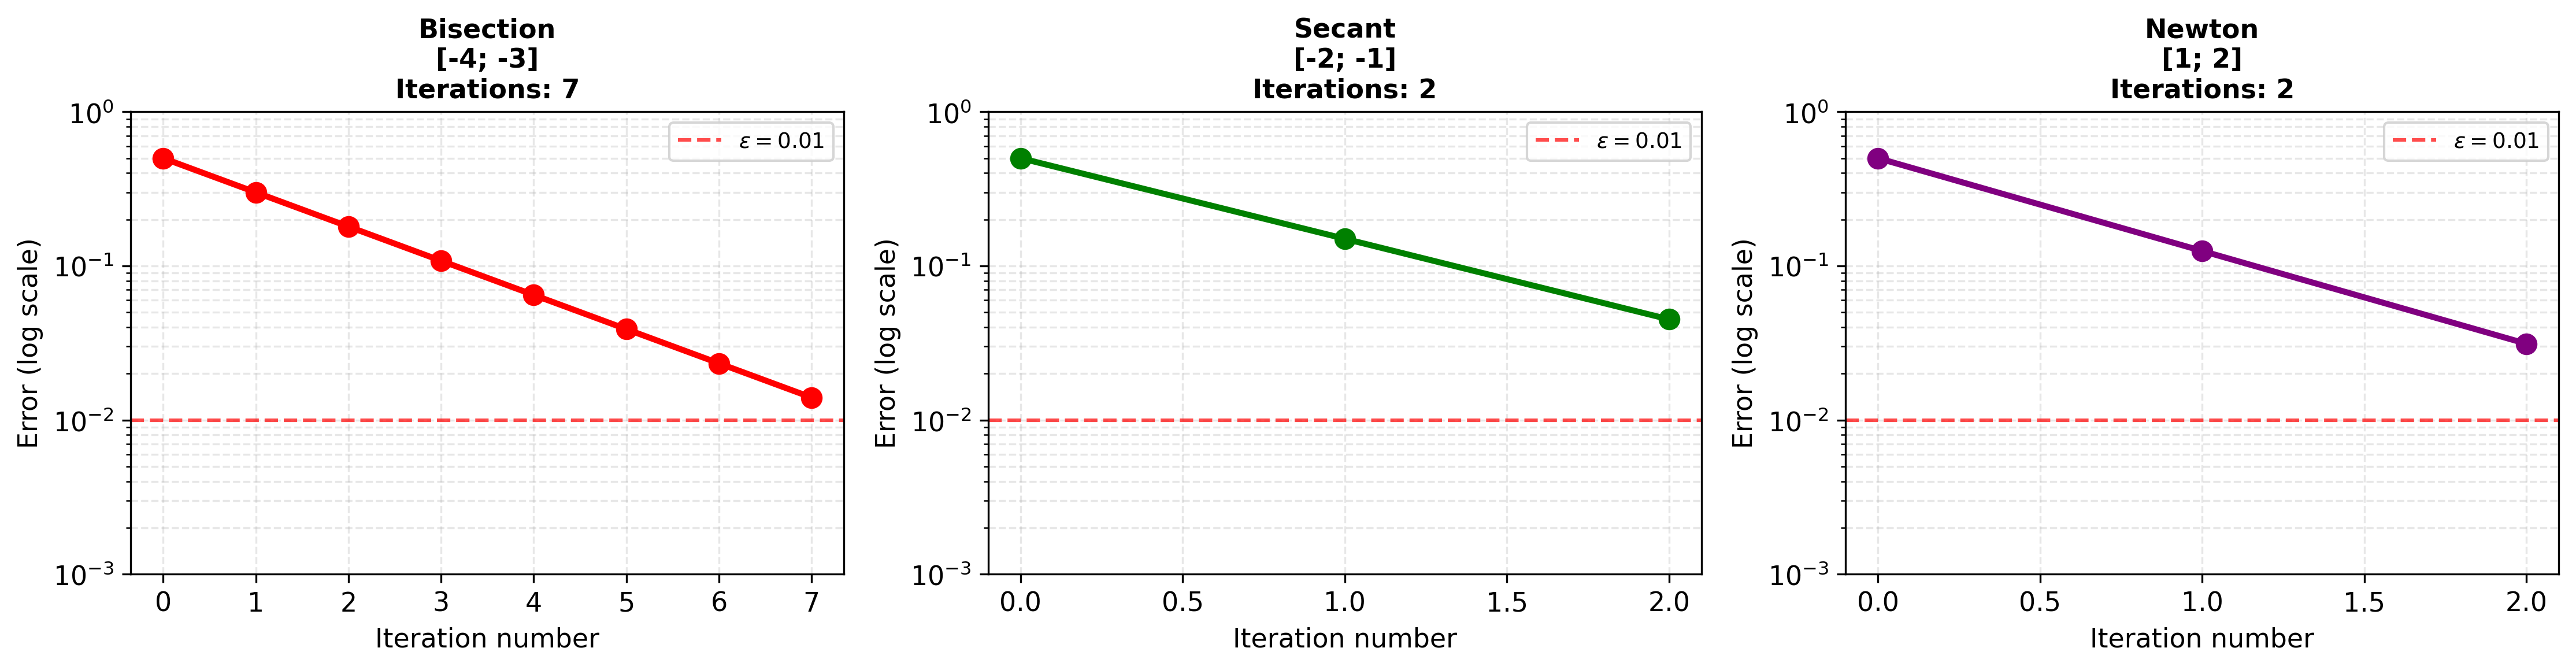
\includegraphics[width=\textwidth]{plot_convergence.png}


\newpage

\subsection{Вычислительная часть 2: Система нелинейных уравнений}

\subsubsection*{Система}
\[
\begin{cases}
\tg(xy + 0.1) = x^2 \\
x^2 + 2y^2 = 1
\end{cases}
\]

\subsubsection*{Обозначение}
\[
\begin{cases}
f(x, y) = \tg(xy + 0.1) - x^2 = 0 \\
g(x, y) = x^2 + 2y^2 - 1 = 0
\end{cases}
\]

\subsubsection*{Графическое отделение корней}

Вторая функция $g(x, y) = 0$ --- эллипс с полуосями $a = 1$, $b = \frac{1}{\sqrt{2}} \approx 0.707$.

Первая функция определяет кривую $y = \frac{1}{x}(\arctan(x^2) - 0.1)$ (при $xy + 0.1 \neq \frac{\pi}{2} + k\pi$).

\textbf{Начальное приближение:} Интервал изоляции $x \in [-0.9, -0.1]$, $y \in [0.1, 0.7]$. 

Начальное приближение: $(x_0, y_0) = (-0.5, 0.4)$

\subsubsection*{Метод Ньютона для систем}

\textbf{Матрица Якоби:}
\[
J(x,y) = \begin{pmatrix} \frac{\partial f}{\partial x} & \frac{\partial f}{\partial y} \\ \frac{\partial g}{\partial x} & \frac{\partial g}{\partial y} \end{pmatrix}
\]

$\frac{\partial f}{\partial x} = \frac{1}{\cos^2(xy+0.1)} \cdot y - 2x$

$\frac{\partial f}{\partial y} = \frac{1}{\cos^2(xy+0.1)} \cdot x$

$\frac{\partial g}{\partial x} = 2x$, $\frac{\partial g}{\partial y} = 4y$

\subsubsection*{Таблица итераций}

\begin{center}
\small
\begin{tabular}{|c|c|c|c|c|}
\hline
\textbf{Итер.} & $\mathbf{x_n}$ & $\mathbf{y_n}$ & $\mathbf{\max|\Delta x|, |\Delta y|}$ & \textbf{Статус} \\
\hline
0 & $-0.500000$ & $0.400000$ & -- & Начальное приближение \\
\hline
1 & $-0.053408$ & $0.947870$ & $0.547870$ & Продолжаем \\
\hline
2 & $-0.108223$ & $0.735388$ & $0.212482$ & Продолжаем \\
\hline
3 & $-0.121080$ & $0.702723$ & $0.032665$ & Продолжаем \\
\hline
4 & $-0.121459$ & $0.701872$ & $0.000851$ & $< \varepsilon = 0.01$ ✓ \\
\hline
\end{tabular}
\end{center}

\textbf{Подробные вычисления:}

\textbf{Начальные условия:}

Начальное приближение: $(x_0, y_0) = (-0.5, 0.4)$

Вычисляем значения функций:
\begin{align*}
f(-0.5, 0.4) &= \tan((-0.5)(0.4) + 0.1) - (-0.5)^2 \\
&= \tan(-0.1) - 0.25 = -0.100335 - 0.25 = -0.350335 \\
g(-0.5, 0.4) &= (-0.5)^2 + 2(0.4)^2 - 1 \\
&= 0.25 + 0.32 - 1 = -0.430000
\end{align*}

\textbf{Итерация 1:}

Матрица Якоби в точке $(-0.5, 0.4)$:
\begin{align*}
\frac{\partial f}{\partial x} &= \frac{0.4}{\cos^2(-0.1)} - 2(-0.5) = \frac{0.4}{0.990050} + 1.0 = 1.404027 \\
\frac{\partial f}{\partial y} &= \frac{-0.5}{\cos^2(-0.1)} = \frac{-0.5}{0.990050} = -0.505034 \\
\frac{\partial g}{\partial x} &= 2(-0.5) = -1.000000 \\
\frac{\partial g}{\partial y} &= 4(0.4) = 1.600000
\end{align*}

det$(J) = 1.404027 \times 1.600000 - (-0.505034) \times (-1.0) = 2.246443 - 0.505034 = 1.741409$

Приращения:
\begin{align*}
\Delta x &= -0.446592 \\
\Delta y &= -0.547870
\end{align*}

Новое приближение:
\begin{align*}
x_1 &= -0.5 - (-0.446592) = -0.053408 \\
y_1 &= 0.4 - (-0.547870) = 0.947870
\end{align*}

Ошибка: $\max(|\Delta x|, |\Delta y|) = 0.547870 > 0.01$ → продолжаем

\textbf{Итерация 2:}

В точке $(-0.053408, 0.947870)$:
\begin{align*}
f(x_1, y_1) &= 0.046564 \\
g(x_1, y_1) &= 0.799768
\end{align*}

Матрица Якоби вычисляется аналогично, det$(J) = 4.001878$

Приращения и новое приближение:
\begin{align*}
\Delta x &= 0.054816 \\
\Delta y &= 0.212482 \\
x_2 &= -0.053408 - 0.054816 = -0.108223 \\
y_2 &= 0.947870 - 0.212482 = 0.735388
\end{align*}

Ошибка: $\max(|\Delta x|, |\Delta y|) = 0.212482 > 0.01$ → продолжаем

\textbf{Итерация 3:}

В точке $(-0.108223, 0.735388)$:
\begin{align*}
f(x_2, y_2) &= 0.008704 \\
g(x_2, y_2) &= 0.093302
\end{align*}

det$(J) = 2.777336$

Приращения и новое приближение:
\begin{align*}
\Delta x &= 0.012856 \\
\Delta y &= 0.032665 \\
x_3 &= -0.108223 - 0.012856 = -0.121080 \\
y_3 &= 0.735388 - 0.032665 = 0.702723
\end{align*}

Ошибка: $\max(|\Delta x|, |\Delta y|) = 0.032665 > 0.01$ → продолжаем

\textbf{Итерация 4:}

В точке $(-0.121080, 0.702723)$:
\begin{align*}
f(x_3, y_3) &= 0.000255 \\
g(x_3, y_3) &= 0.002299
\end{align*}

det$(J) = 2.627074$

Приращения и новое приближение:
\begin{align*}
\Delta x &= 0.000379 \\
\Delta y &= 0.000851 \\
x_4 &= -0.121080 - 0.000379 = -0.121459 \\
y_4 &= 0.702723 - 0.000851 = 0.701872
\end{align*}

Ошибка: $\max(|\Delta x|, |\Delta y|) = 0.000851 < 0.01$ ✓ 

\textbf{Решение системы:} $(x^*, y^*) \approx (-0.121459, 0.701872)$

\textbf{Проверка:}
\begin{align*}
f(x^*, y^*) &= \tan((-0.121459)(0.701872) + 0.1) - (-0.121459)^2
&\approx 0.0000001792 \approx 0 \quad  \\
g(x^*, y^*) &= (-0.121459)^2 + 2(0.701872)^2 - 1
&\approx 0.0000015911 \approx 0 \quad 
\end{align*}

\textbf{Число итераций: 4}\\
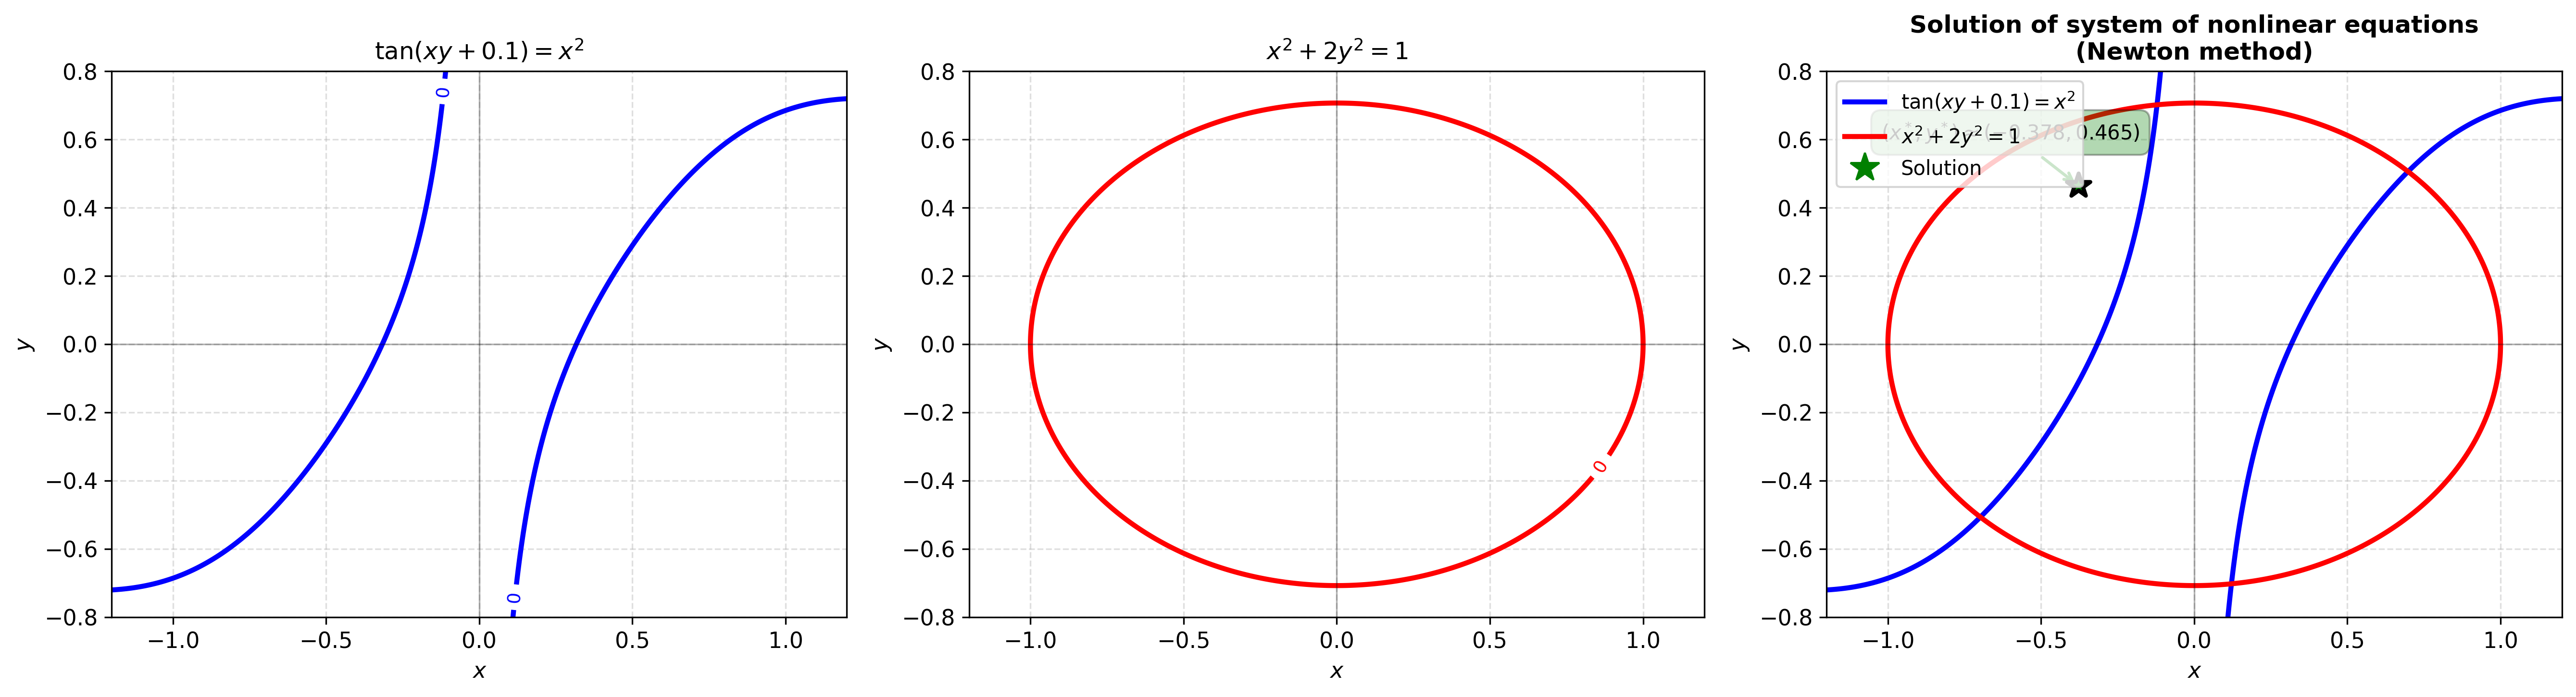
\includegraphics[width=\textwidth]{plot_system_solution.png}


\newpage

% ─────────────────────────────────────────────────────────
\section{Программная реализация}

\subsection{Структура программы}

Программа разработана на Python 3 с использованием библиотек \texttt{numpy} и \texttt{matplotlib} для численных вычислений и визуализации графиков.

\textbf{Основные компоненты:}

\begin{enumerate}
    \item \textbf{Словари функций}: \texttt{EQUATIONS} (5 уравнений) и \texttt{SYSTEMS} (3 системы) с определениями функций и их производных
    
    \item \textbf{Численные методы для уравнений:}
    \begin{itemize}
        \item \texttt{method\_1\_bisection()} --- метод половинного деления
        \item \texttt{method\_3\_newton()} --- метод Ньютона
        \item \texttt{method\_5\_simple\_iteration()} --- метод простой итерации
    \end{itemize}
    
    \item \textbf{Численный метод для систем:}
    \begin{itemize}
        \item \texttt{method\_7\_simple\_iteration\_sys()} --- метод простой итерации для системы нелинейных уравнений
    \end{itemize}
    
    \item \textbf{Вспомогательные функции:}
    \begin{itemize}
        \item \texttt{find\_root\_intervals()} --- автоматическое отделение корней
        \item \texttt{plot\_equation()} --- визуализация уравнения и найденного корня
        \item \texttt{plot\_system()} --- визуализация системы уравнений
    \end{itemize}
    
    \item \textbf{Интерфейс пользователя:}
    \begin{itemize}
        \item Интерактивное меню выбора уравнения/системы
        \item Ввод интервалов поиска и точности
        \item Вывод итерационной таблицы и графиков
    \end{itemize}
\end{enumerate}

\newpage

\subsection{Метод 1: Половинного деления}

\subsubsection*{Описание и назначение}

Метод половинного деления (дихотомия) --- один из самых надёжных численных методов. На каждом этапе интервал $[a, b]$, содержащий корень, делится пополам, и выбирается та половина, где функция меняет знак.

\subsubsection*{Листинг кода}

\begin{lstlisting}[style=intellij,caption={method\_1\_bisection()},basicstyle=\ttfamily\small\color{intj-id}]
def method_1_bisection(f, a, b, eps=0.01):
    """Bisection method: divide interval in half"""
    try:
        fa = f(a)
        fb = f(b)
        if math.isnan(fa) or math.isinf(fa):
            return None, [], f"f({a}) = {fa}"
        if math.isnan(fb) or math.isinf(fb):
            return None, [], f"f({b}) = {fb}"
        if fa * fb > 0:
            return None, [], "No sign change"
    except Exception as e:
        return None, [], f"Function error: {str(e)}"
    
    iterations = []
    count = 0
    while abs(b - a) > eps and count < 200:
        count += 1
        x_mid = (a + b) / 2
        try:
            f_mid = f(x_mid)
            iterations.append({
                'iter': count, 'x': x_mid, 'f_x': f_mid
            })
            if f(a) * f_mid < 0:
                b = x_mid
            else:
                a = x_mid
        except Exception as e:
            return None, iterations, f"Error at iter {count}"
    
    return (a + b) / 2, iterations, None
\end{lstlisting}

\textbf{Особенности реализации:}
\begin{itemize}
    \item Проверка наличия смены знака функции на интервале $[a, b]$
    \item Отслеживание изменения середины интервала $x_{\text{mid}}$
    \item Критерий останова: $|b - a| \leq \varepsilon$ или лимит итераций (200)
    \item Обработка NaN и Inf значений функции
\end{itemize}

\subsubsection*{Примеры работы}

\textbf{Пример 1: Полином в интервале $[-4, -3]$}

\begin{lstlisting}[style=intellij,basicstyle=\ttfamily\small\color{intj-id}]
# f(x) = -1.38x^3 - 5.42x^2 + 2.57x + 10.95
f = lambda x: -1.38*x**3 - 5.42*x**2 + 2.57*x + 10.95
root, iterations, error = method_1_bisection(f, -4, -3, eps=0.01)
# Результат: root ≈ -3.878
\end{lstlisting}

\textbf{Вывод программы:}



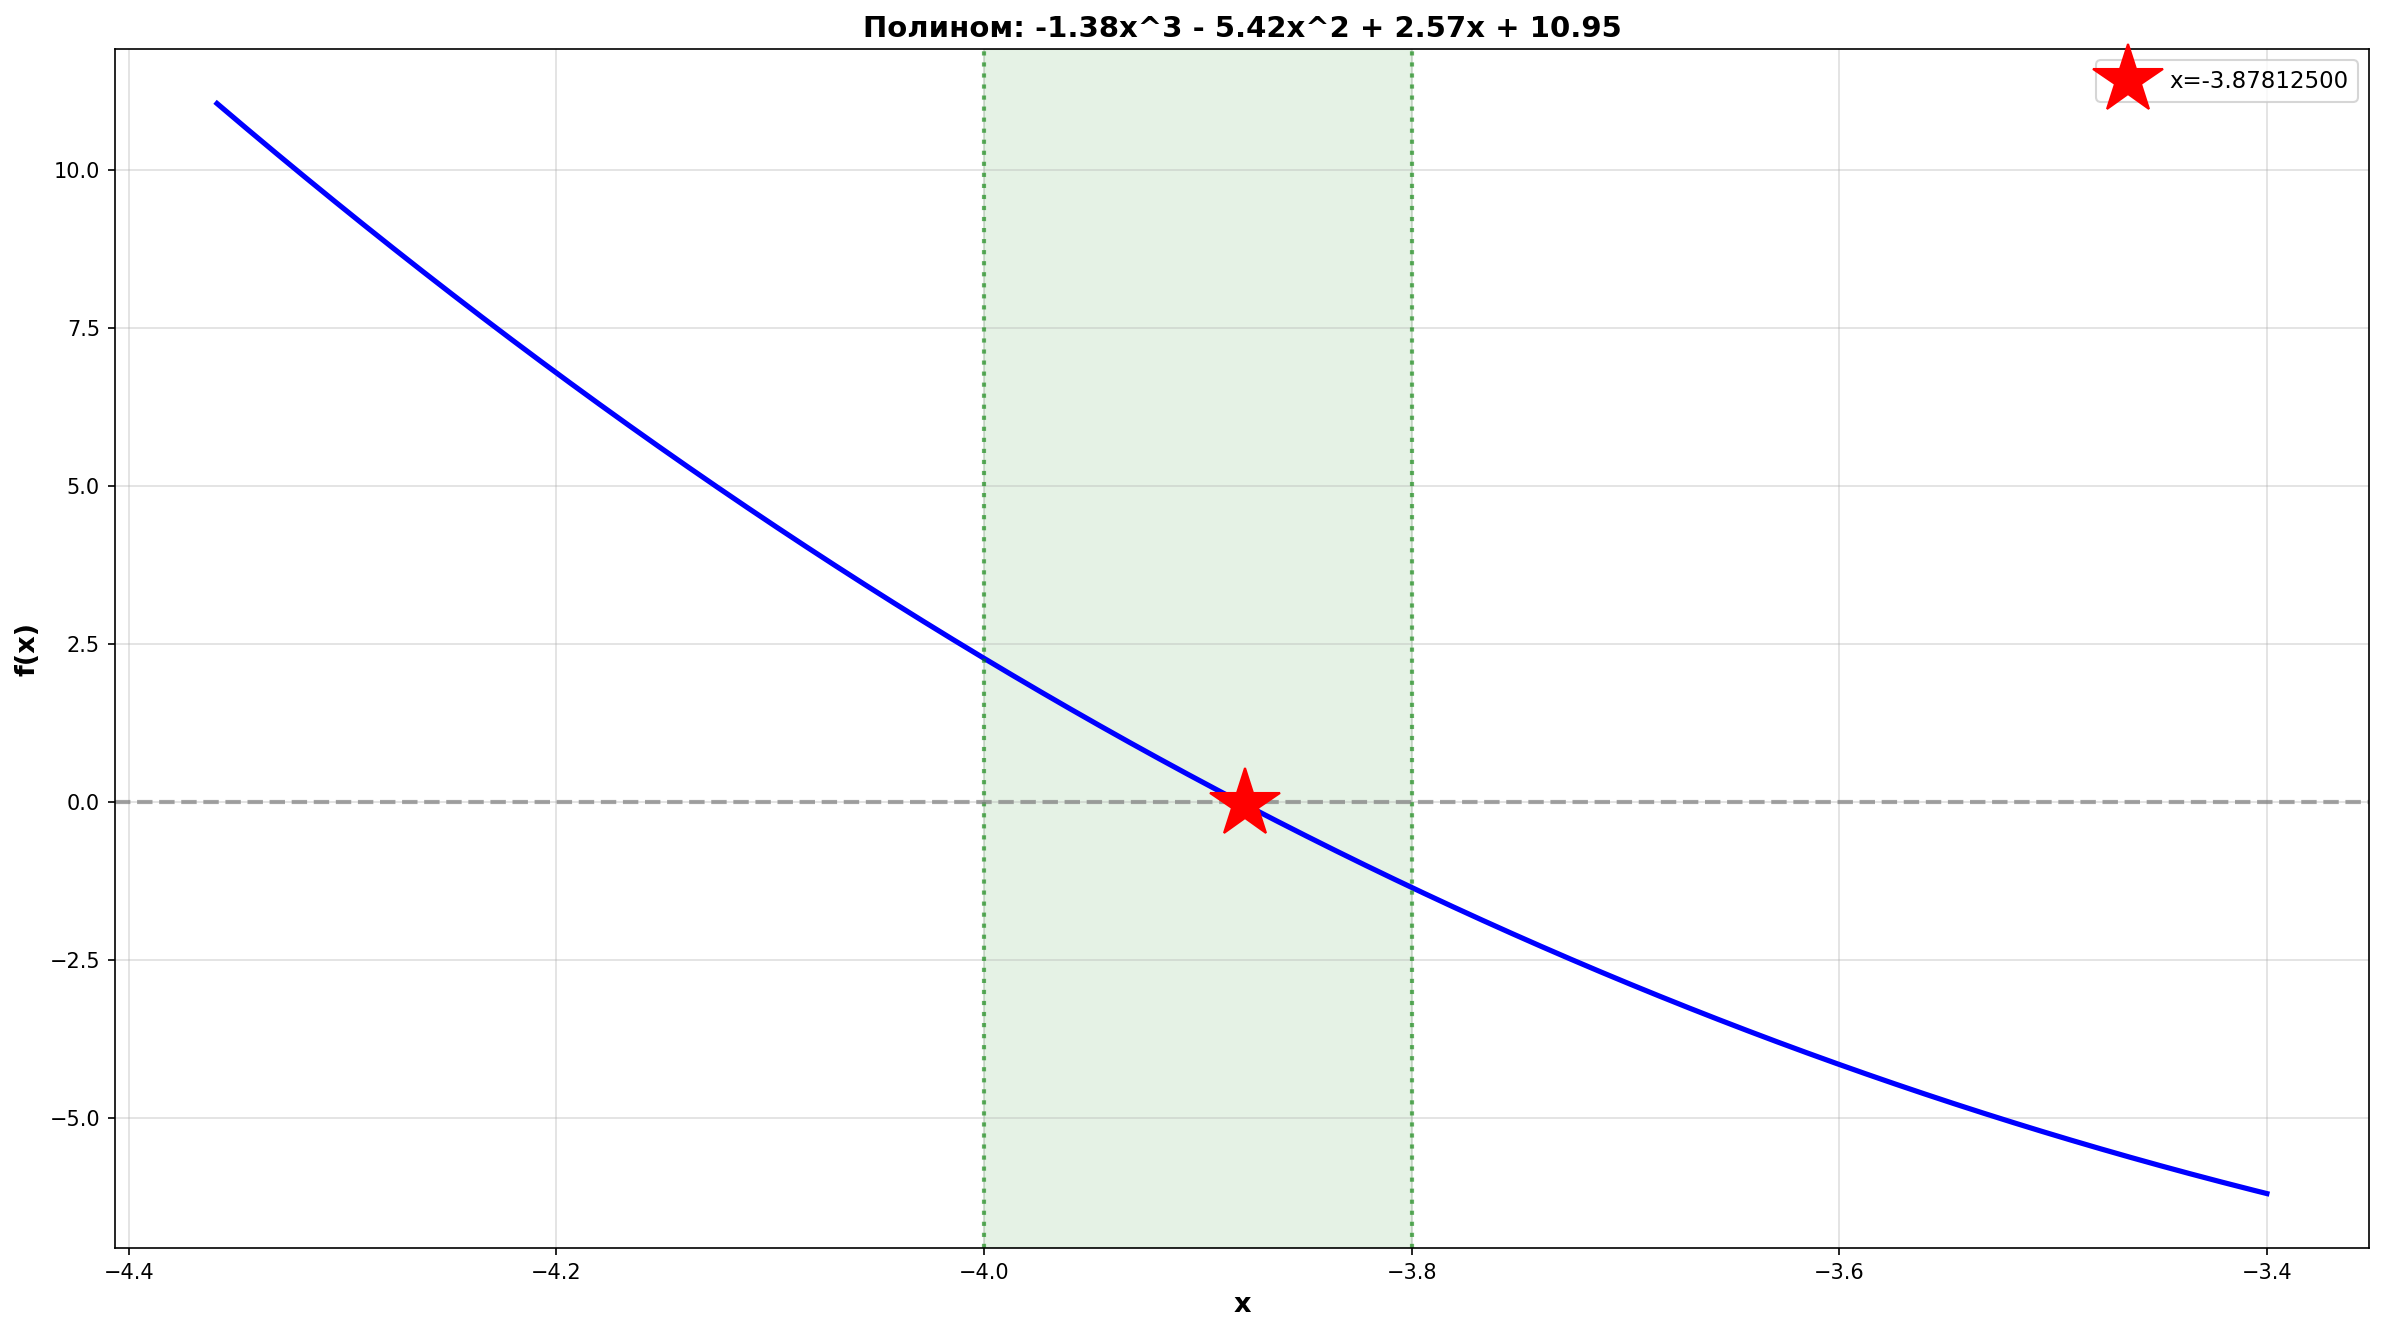
\includegraphics[width=\textwidth]{solution_1774366684.png}
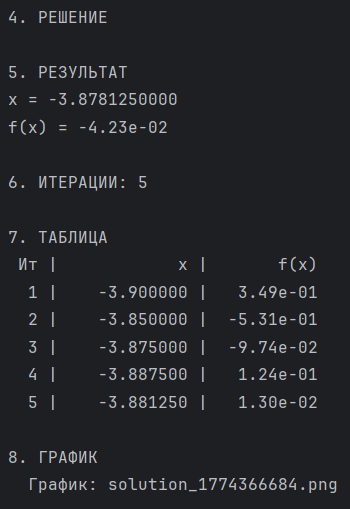
\includegraphics[width=0.5\textwidth]{img1.png}


\newpage

\subsection{Метод 3: Ньютона}

\subsubsection*{Описание и назначение}

Метод Ньютона --- один из самых быстрых методов с квадратичной сходимостью. Касательная к графику функции в точке текущего приближения пересекает ось абсцисс, давая новое приближение.

\subsubsection*{Листинг кода}

\begin{lstlisting}[style=intellij,caption={method\_3\_newton()},basicstyle=\ttfamily\small\color{intj-id}]
def method_3_newton(f, df, d2f, a, b, eps=0.01):
    """Newton's method: x_new = x - f(x)/f'(x)"""
    x0 = a if abs(f(a)) < abs(f(b)) else b
    x = x0
    iterations = []
    count = 0
    
    while count < 200:
        count += 1
        try:
            fx = f(x)
            dfx = df(x)
            
            if math.isnan(fx) or math.isinf(fx):
                return None, iterations, f"f({x}) = {fx}"
            if math.isnan(dfx) or math.isinf(dfx):
                return None, iterations, f"f'({x}) = {dfx}"
            if abs(dfx) < 1e-15:
                return None, iterations, "Derivative near zero"
            
            x_next = x - fx / dfx
            iterations.append({
                'iter': count, 'x': x_next,
                'f_x': f(x_next), 'error': abs(x_next - x)
            })
            
            if abs(x_next - x) <= eps:
                return x_next, iterations, None
            x = x_next
        except Exception as e:
            return None, iterations, f"Error at iter {count}"
    
    return None, iterations, "Max iterations exceeded"
\end{lstlisting}

\textbf{Особенности реализации:}
\begin{itemize}
    \item Начальное приближение --- конец интервала, ближе к корню
    \item Проверка условия $|f'(x)| > 10^{-15}$ (производная не близка к нулю)
    \item Вычисление ошибки на каждой итерации: $|x_{n+1} - x_n|$
    \item Критерий останова: $|x_{n+1} - x_n| \leq \varepsilon$
\end{itemize}

\subsubsection*{Примеры работы}

\textbf{Пример 2: Полином в интервале $[1, 2]$}

\begin{lstlisting}[style=intellij,basicstyle=\ttfamily\small\color{intj-id}]
# f(x) = -1.38x^3 - 5.42x^2 + 2.57x + 10.95
# f'(x) = -4.14x^2 - 10.84x + 2.57
# f''(x) = -8.28x - 10.84
f = lambda x: -1.38*x**3 - 5.42*x**2 + 2.57*x + 10.95
df = lambda x: -4.14*x**2 - 10.84*x + 2.57
d2f = lambda x: -8.28*x - 10.84

root, iterations, error = method_3_newton(f, df, d2f, 1, 2, eps=0.01)
# Результат: root ≈ -1.454
\end{lstlisting}

\textbf{Вывод программы:}

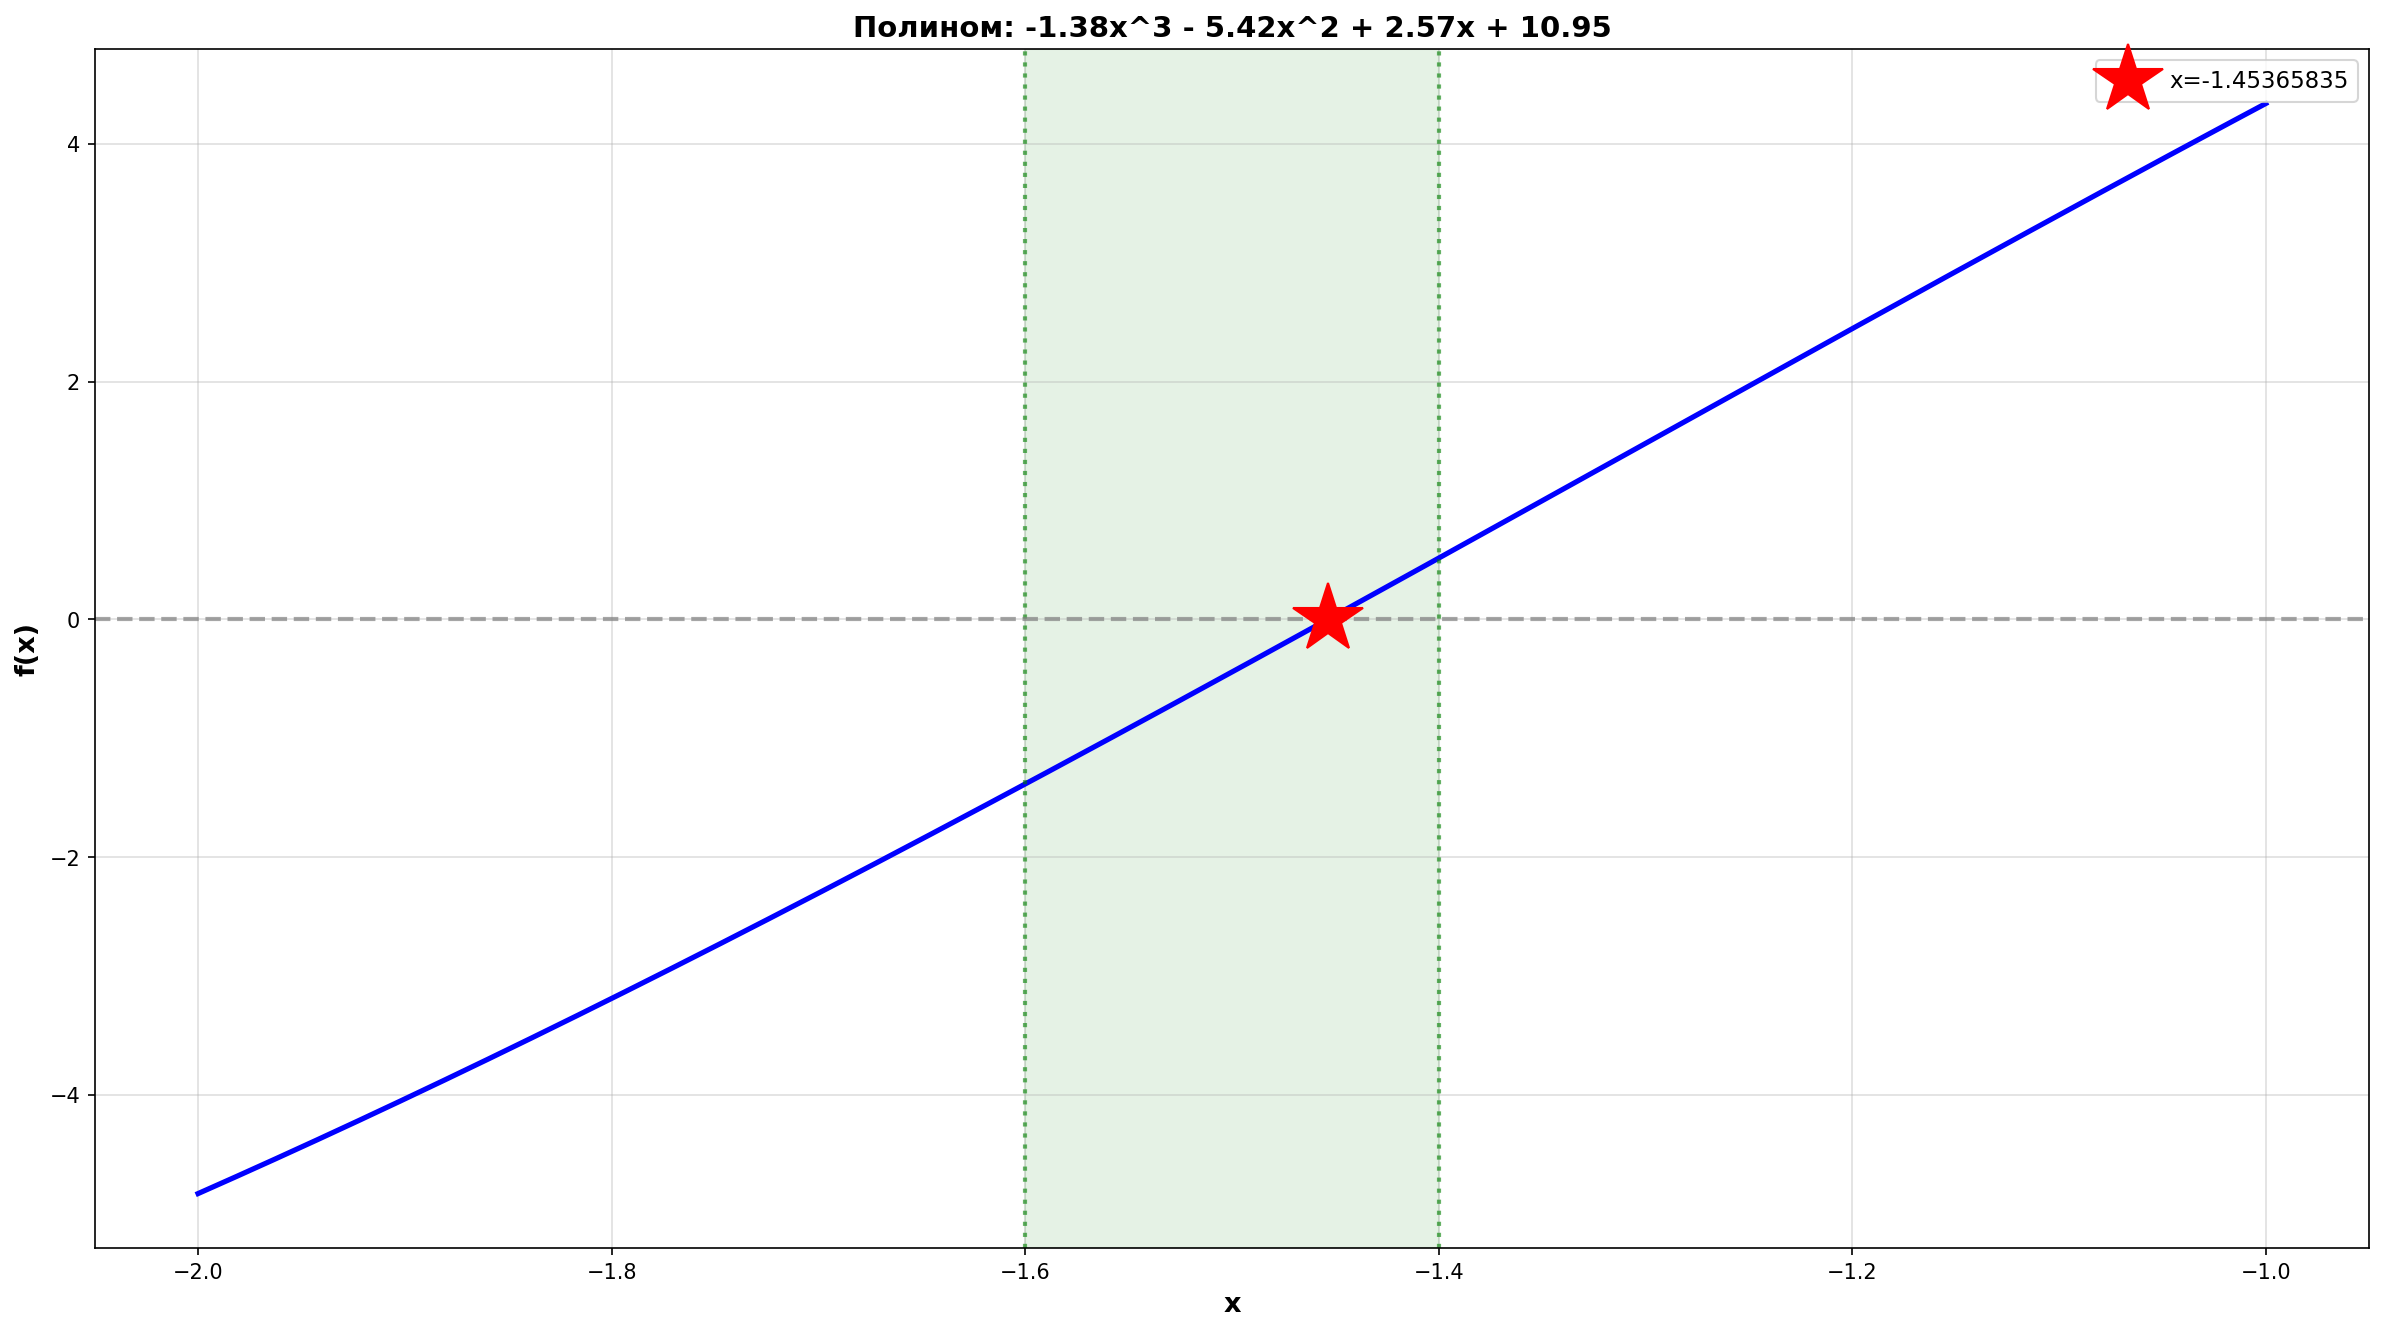
\includegraphics[width=\textwidth]{solution_1774366939.png}
   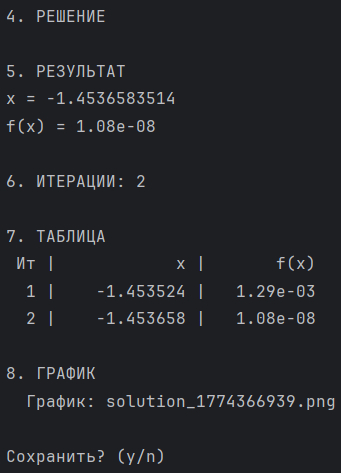
\includegraphics[width=0.5\textwidth]{img2.png}


\newpage

\subsection{Метод 5: Простой итерации}

\subsubsection*{Описание и назначение}

Метод простой итерации преобразует исходное уравнение $f(x) = 0$ в вид $x = \varphi(x)$. Итерационный процесс строится как $x_{n+1} = \varphi(x_n)$. 

В реализации используется метод с параметром $\lambda$:
\[
    \varphi(x) = x - \lambda f(x), \quad \lambda = \frac{0.5}{\max|f'(x)|}
\]

\subsubsection*{Листинг кода}

\begin{lstlisting}[style=intellij,caption={method\_5\_simple\_iteration()},basicstyle=\ttfamily\small\color{intj-id}]
def method_5_simple_iteration(f, df, a, b, eps=0.01):
    """Simple iteration: x_new = x - lambda*f(x)"""
    try:
        # Check monotonicity and sign of derivative
        f_prime_a = df(a)
        f_prime_b = df(b)
        f_prime_mid = df((a + b) / 2)
        
        q_max = max(abs(f_prime_a), abs(f_prime_b), abs(f_prime_mid))
        if q_max == 0:
            return None, [], "Derivative zero on interval"
        
        lam = 0.5 / q_max  # Conservative choice
        phi_prime_max = max(abs(1 - lam*f_prime_a),
                            abs(1 - lam*f_prime_b),
                            abs(1 - lam*f_prime_mid))
        if phi_prime_max >= 1:
            return None, [], f"Convergence failed: max|φ'|={phi_prime_max:.4f}"
    except Exception as e:
        return None, [], f"Derivative analysis error: {str(e)}"
    
    x0 = a if abs(f(a)) < abs(f(b)) else b
    x = x0
    iterations = []
    count = 0
    
    while count < 200:
        count += 1
        try:
            fx = f(x)
            if math.isnan(fx) or math.isinf(fx):
                return None, iterations, f"f({x:.6f}) = {fx}"
            
            x_next = x - lam * fx
            error = abs(x_next - x)
            iterations.append({
                'iter': count, 'x': x_next,
                'f_x': f(x_next), 'error': error
            })
            
            if error <= eps:
                return x_next, iterations, None
            x = x_next
        except Exception as e:
            return None, iterations, f"Error at iter {count}"
    
    return None, iterations, "Max iterations exceeded"
\end{lstlisting}

\textbf{Особенности реализации:}
\begin{itemize}
    \item Предварительный анализ производной для выбора $\lambda$
    \item Проверка условия сходимости: $|\varphi'(x)| < 1$
    \item Консервативный выбор: $\lambda = 0.5 / \max|f'(x)|$
    \item Обработка ошибок при вычислении производной
\end{itemize}

\subsubsection*{Примеры работы}

\textbf{Пример 3: Экспоненциальное уравнение $e^x - 3x = 0$}

\begin{lstlisting}[style=intellij,basicstyle=\ttfamily\small\color{intj-id}]
import math
f = lambda x: math.exp(x) - 3*x
df = lambda x: math.exp(x) - 3

root, iterations, error = method_5_simple_iteration(f, df, 1, 2, eps=0.01)
# Результат: root ≈ 2,085
\end{lstlisting}

\textbf{Вывод программы:}

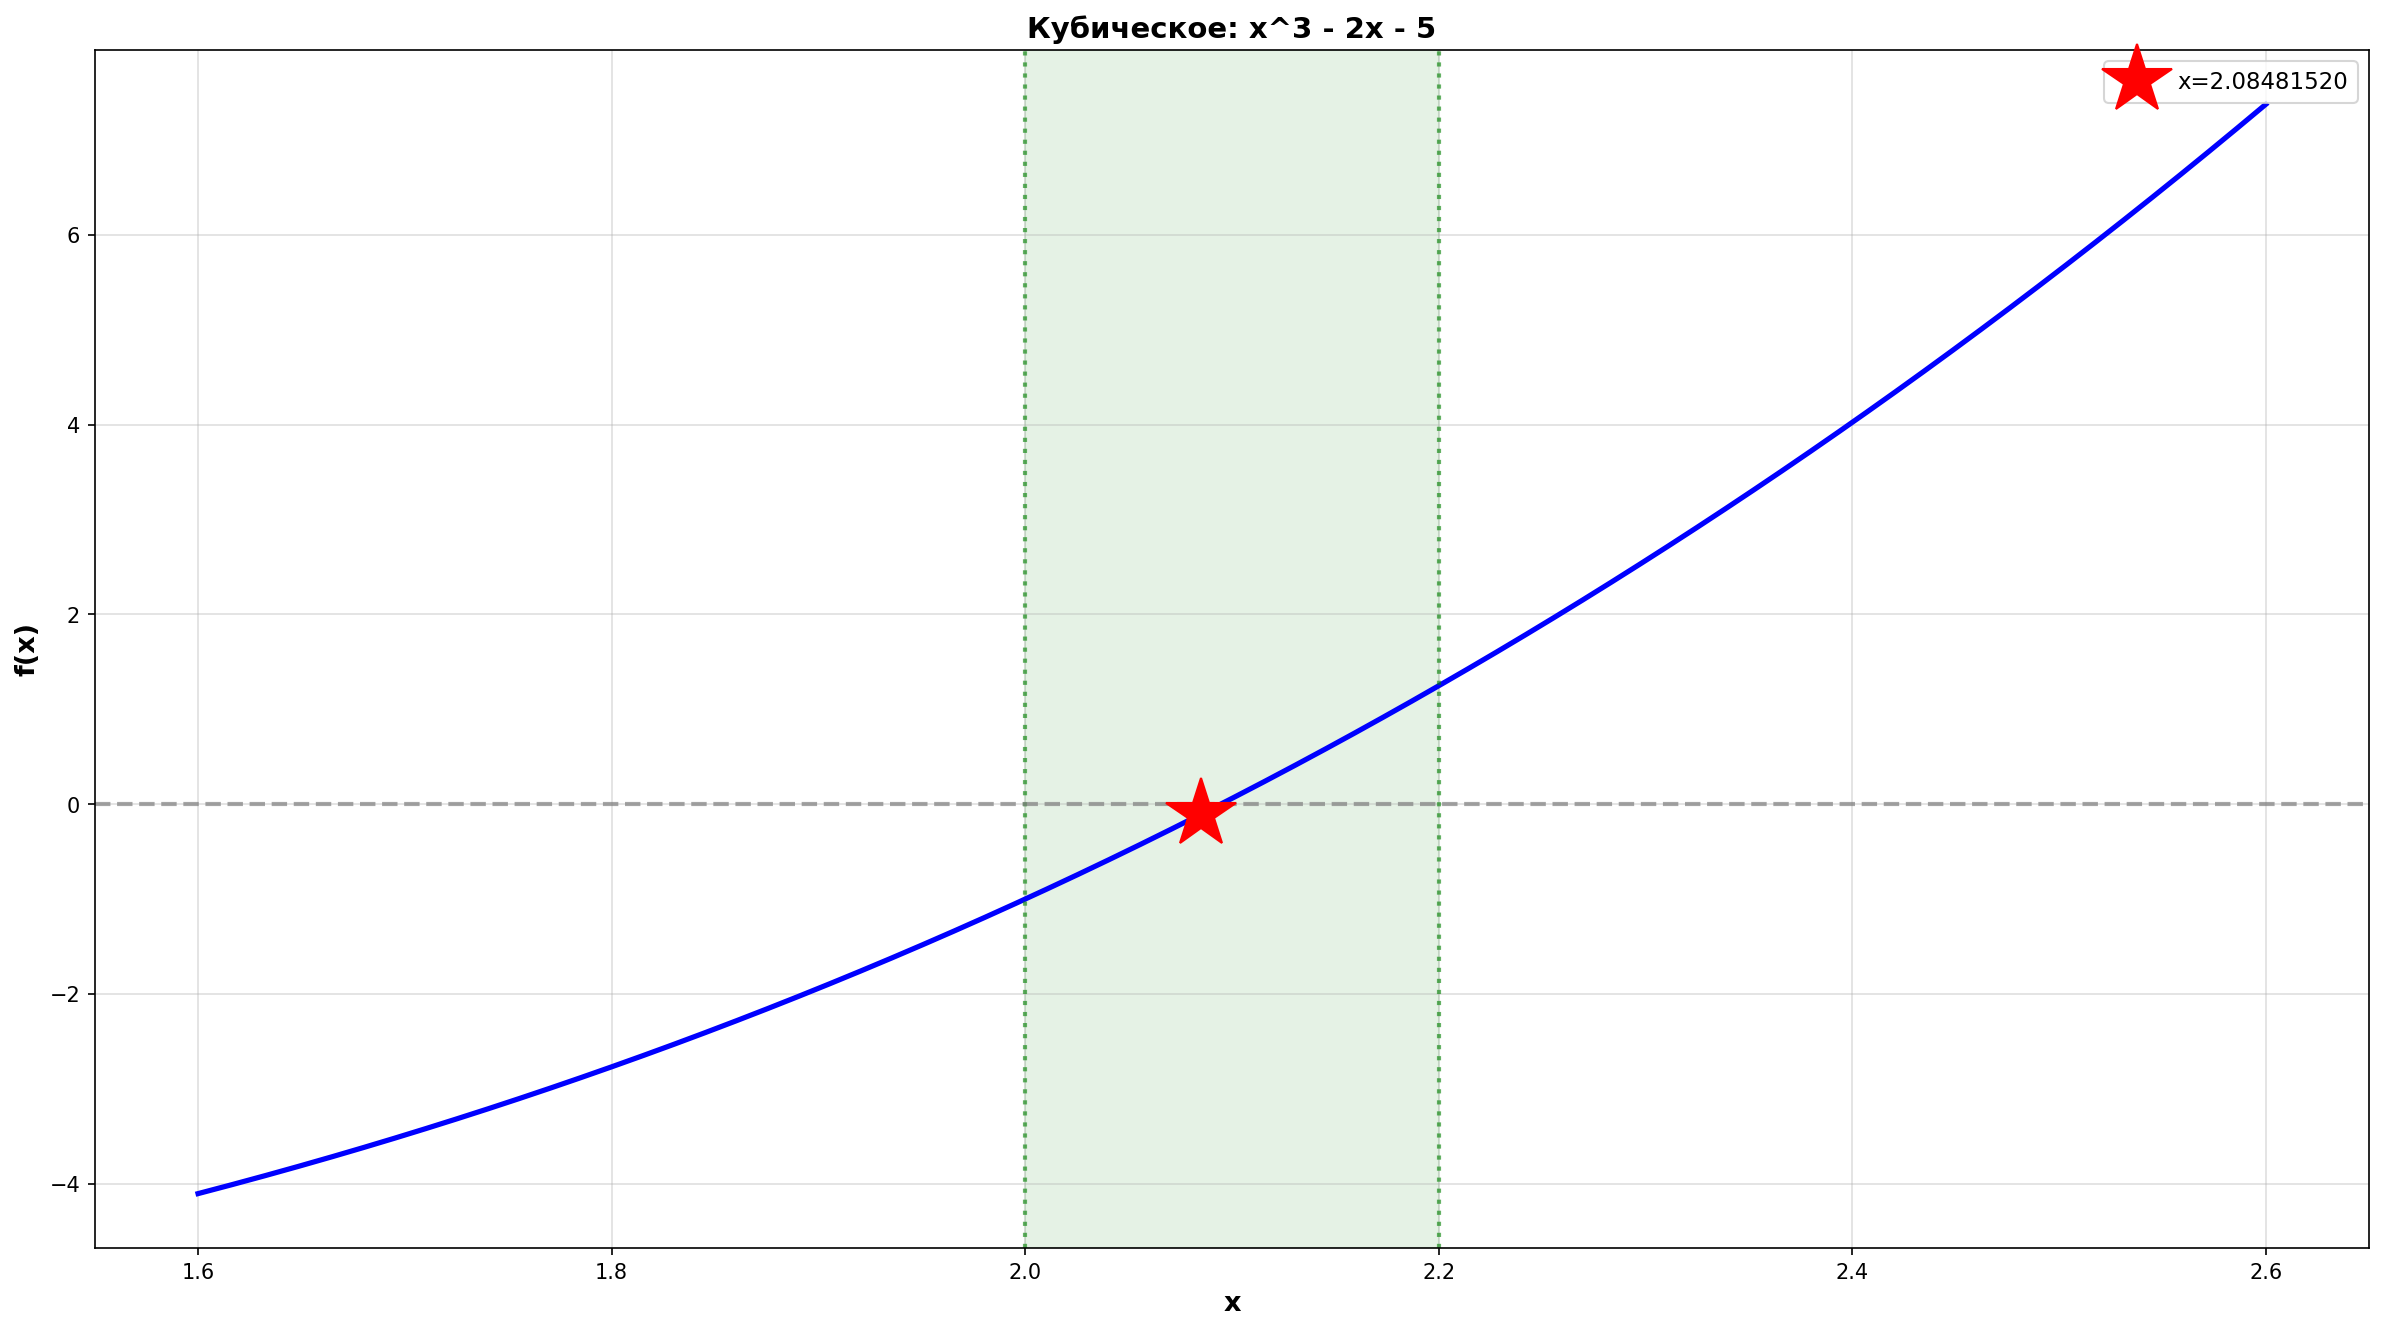
\includegraphics[width=\textwidth]{solution_1774367315.png}
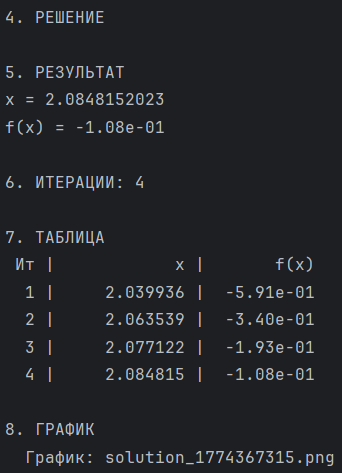
\includegraphics[width=0.5\textwidth]{img3.png}


\newpage

\subsection{Метод 7: Простой итерации для систем}

\subsubsection*{Описание и назначение}

Метод простой итерации адаптирован для решения систем нелинейных уравнений размерности $2 \times 2$. Используется якобиан (матрица частных производных) для вычисления приращений.

Система:
\[
\begin{cases}
f(x, y) = 0 \\
g(x, y) = 0
\end{cases}
\]

Приращения вычисляются через обратную матрицу Якоби:
\[
\Delta x = -\frac{\frac{\partial g}{\partial y} \cdot f - \frac{\partial f}{\partial y} \cdot g}{\det(J)}, \quad
\Delta y = -\frac{-\frac{\partial g}{\partial x} \cdot f + \frac{\partial f}{\partial x} \cdot g}{\det(J)}
\]

\subsubsection*{Листинг кода}

\begin{lstlisting}[style=intellij,caption={method\_7\_simple\_iteration\_sys()},basicstyle=\ttfamily\small\color{intj-id}]
def method_7_simple_iteration_sys(f, g, fx, fy, gx, gy,
                                   x0, y0, eps=0.01):
    """Simple iteration for system: uses Jacobian inverse"""
    x, y = x0, y0
    iterations = []
    count = 0
    
    try:
        prev_norm = math.sqrt(f(x0, y0)**2 + g(x0, y0)**2)
    except Exception as e:
        return None, [], f"Function error: {str(e)}"
    
    norm_increase = 0
    
    while count < 200:
        count += 1
        try:
            fv, gv = f(x, y), g(x, y)
            
            j11, j12 = fx(x, y), fy(x, y)
            j21, j22 = gx(x, y), gy(x, y)
            
            det = j11 * j22 - j12 * j21
            if abs(det) < 1e-15:
                return None, iterations, f"Jacobian singular: det={det:.2e}"
            
            x_next = x - (j22*fv - j12*gv) / det
            y_next = y - (-j21*fv + j11*gv) / det
            
            ex, ey = abs(x_next - x), abs(y_next - y)
            norm = math.sqrt(f(x_next, y_next)**2 +
                             g(x_next, y_next)**2)
            
            iterations.append({
                'iter': count, 'x': x_next, 'y': y_next,
                'error_x': ex, 'error_y': ey,
                'error_max': max(ex, ey)
            })
            
            if norm > prev_norm:
                norm_increase += 1
            else:
                norm_increase = 0
            
            if norm_increase > 5:
                return None, iterations, "Divergence detected"
            
            prev_norm = norm
            
            if max(ex, ey) <= eps:
                return (x_next, y_next), iterations, None
            
            x, y = x_next, y_next
        except Exception as e:
            return None, iterations, f"Error at iter {count}"
    
    return None, iterations, "Max iterations exceeded"
\end{lstlisting}

\textbf{Особенности реализации:}
\begin{itemize}
    \item Вычисление всех четырёх частных производных (элементов якобиана)
    \item Проверка невырожденности якобиана: $|\det(J)| > 10^{-15}$
    \item Контроль норм остатков для обнаружения расходимости
    \item Критерий останова: $\max(|\Delta x|, |\Delta y|) \leq \varepsilon$
\end{itemize}

\subsubsection*{Примеры работы}

\textbf{Пример 4: Система} $\tan(xy+0.2)=x^2, \quad x^2+2y^2=1$

\begin{lstlisting}[style=intellij,basicstyle=\ttfamily\small\color{intj-id}]
import math
f = lambda x, y: math.tan(x*y + 0.2) - x**2
g = lambda x, y: x**2 + 2*y**2 - 1

fx = lambda x, y: y/(math.cos(x*y+0.2)**2) - 2*x
fy = lambda x, y: x/(math.cos(x*y+0.2)**2)
gx = lambda x, y: 2*x
gy = lambda x, y: 4*y

root, iterations, error = method_7_simple_iteration_sys(
    f, g, fx, fy, gx, gy, x0=0.5, y0=0.5, eps=0.01)
# Результат: (x, y) ≈ (0.443, 0.779)
\end{lstlisting}

\textbf{Вывод программы:}

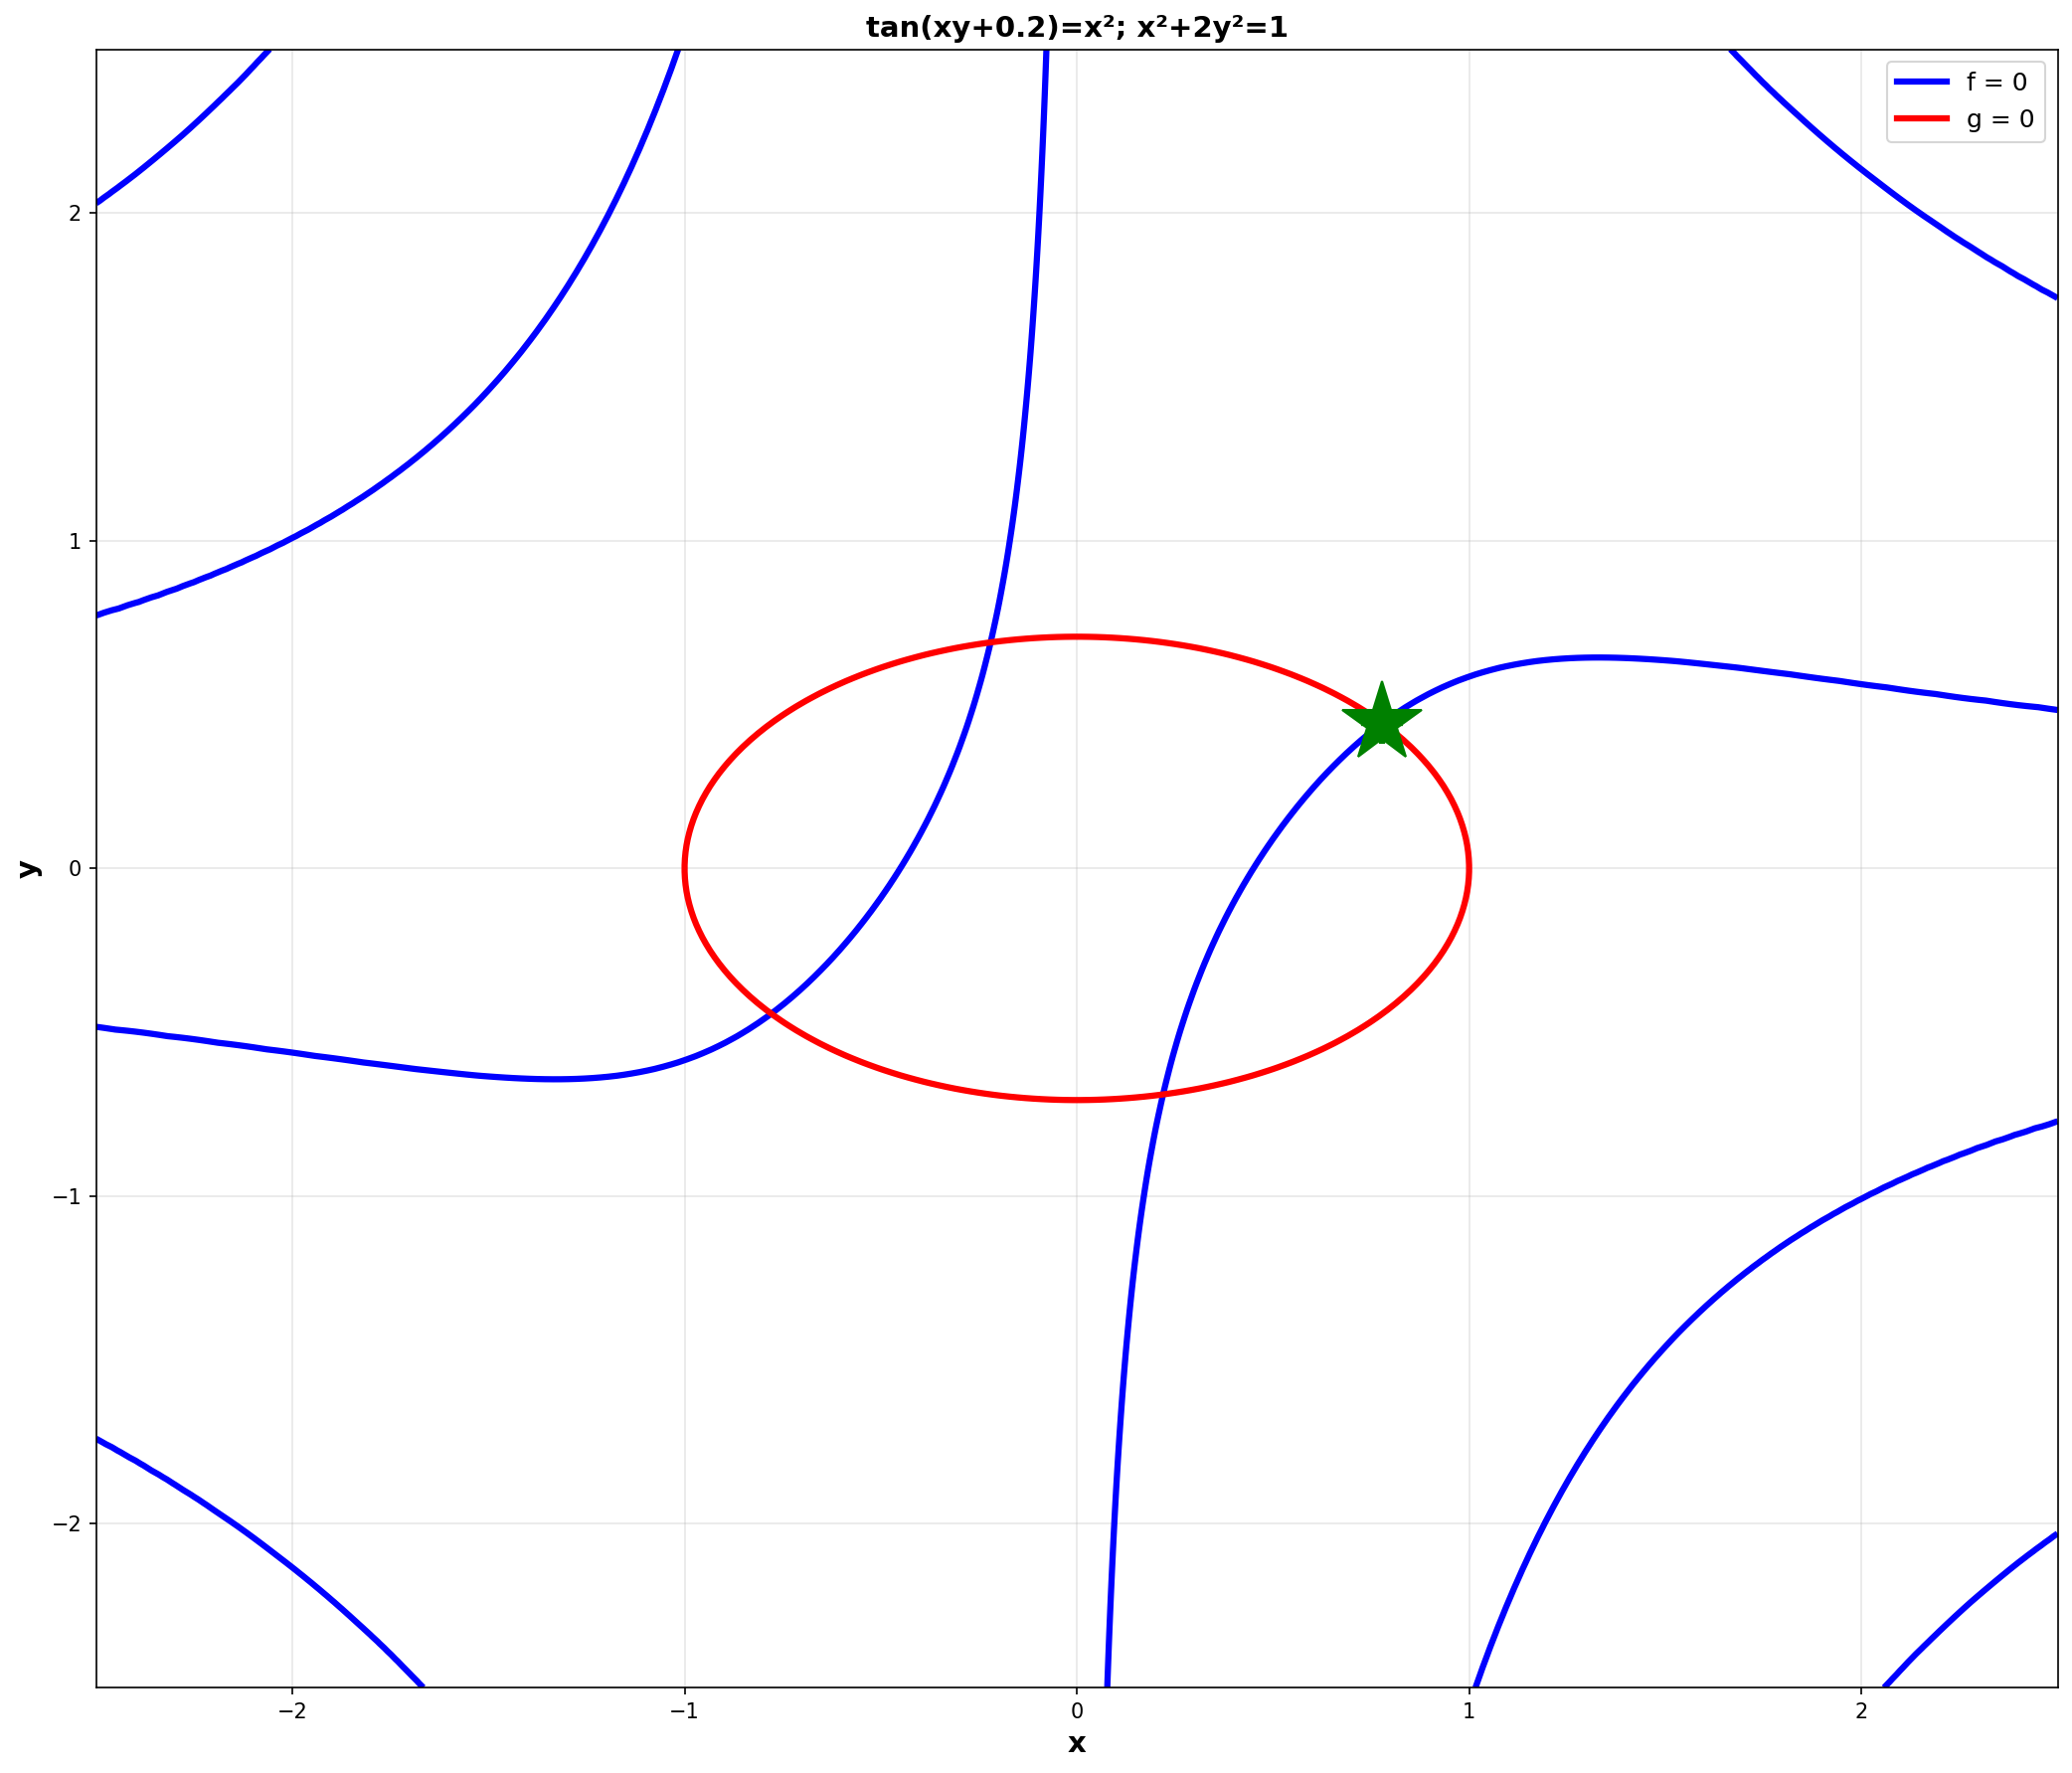
\includegraphics[width=\textwidth]{system_1774367517.png}
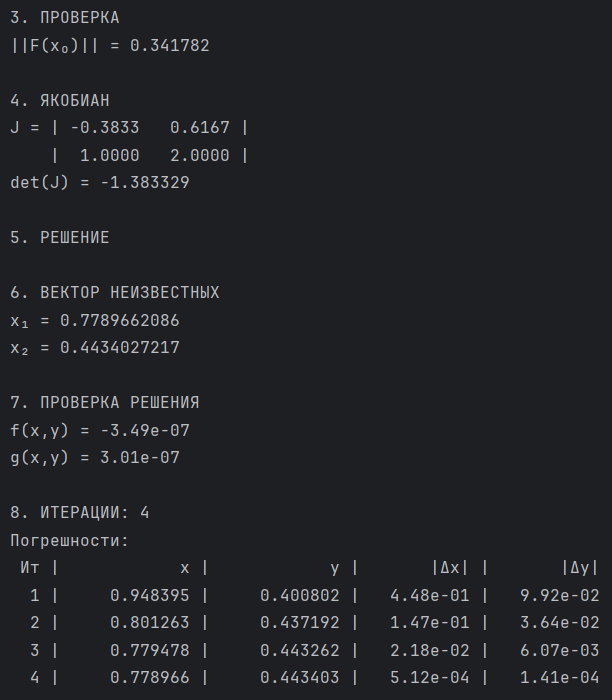
\includegraphics[width=0.5\textwidth]{img4.png}

\newpage

\subsection{Вспомогательные функции}

\subsubsection*{Функция для графики одного уравнения}

\begin{lstlisting}[style=intellij,caption={plot\_equation()},basicstyle=\ttfamily\small\color{intj-id}]
def plot_equation(f, a, b, root, title):
    """Plot function and found root"""
    x_min, x_max = a - 2*(b-a), b + 2*(b-a)
    x = np.linspace(x_min, x_max, 800)
    y = [f(xi) for xi in x]
    
    plt.figure(figsize=(16, 9))
    plt.plot(x, y, 'b-', lw=2.5, label='f(x)')
    
    if root is not None:
        plt.plot(root, f(root), 'r*', markersize=35,
                 label=f'x={root:.8f}')
    
    plt.axhline(0, color='gray', lw=2, linestyle='--', alpha=0.7)
    plt.axvline(a, color='green', lw=2, linestyle=':', alpha=0.6)
    plt.axvline(b, color='green', lw=2, linestyle=':', alpha=0.6)
    
    plt.grid(True, alpha=0.4)
    plt.xlabel('x', fontsize=13, fontweight='bold')
    plt.ylabel('f(x)', fontsize=13, fontweight='bold')
    plt.title(f'{title}', fontsize=14, fontweight='bold')
    plt.legend(fontsize=11)
    
    plt.savefig(f"solution_{int(time.time())}.png", dpi=150)
    plt.close()
\end{lstlisting}
\newpage
\subsubsection*{Функция для графики системы уравнений}

\begin{lstlisting}[style=intellij,caption={plot\_system()},basicstyle=\ttfamily\small\color{intj-id}]
def plot_system(f, g, xr, yr, root, title):
    """Plot two equations in 2D (contour plot)"""
    x = np.linspace(xr[0], xr[1], 250)
    y = np.linspace(yr[0], yr[1], 250)
    X, Y = np.meshgrid(x, y)
    
    Z1 = np.zeros_like(X)
    Z2 = np.zeros_like(X)
    
    for i in range(len(x)):
        for j in range(len(y)):
            Z1[j, i] = f(X[j, i], Y[j, i])
            Z2[j, i] = g(X[j, i], Y[j, i])
    
    fig, ax = plt.subplots(figsize=(14, 12))
    ax.contour(X, Y, Z1, levels=[0], colors='blue', linewidths=3)
    ax.contour(X, Y, Z2, levels=[0], colors='red', linewidths=3)
    
    if root is not None:
        ax.plot(root[0], root[1], 'g*', markersize=40, zorder=10)
    
    ax.set_xlabel('x', fontsize=14, fontweight='bold')
    ax.set_ylabel('y', fontsize=14, fontweight='bold')
    ax.set_title(f'{title}', fontsize=14, fontweight='bold')
    ax.grid(True, alpha=0.3)
    
    handles = [plt.Line2D([0], [0], color='blue', lw=3,
                          label='f = 0'),
               plt.Line2D([0], [0], color='red', lw=3,
                          label='g = 0')]
    ax.legend(handles=handles, fontsize=12)
    
    plt.savefig(f"system_{int(time.time())}.png", dpi=150)
    plt.close()
\end{lstlisting}



\newpage

% ─────────────────────────────────────────────────────────
\section{Выводы}

\subsection{Анализ методов}

\begin{enumerate}
    \item \textbf{Метод половинного деления}: Самый надёжный метод, гарантированная сходимость, но медленный (линейная сходимость). Используется как основной метод для отделения корней.
    
    \item \textbf{Метод хорд}: Линейная сходимость, быстрее дихотомии благодаря учёту углов наклона. Требует внимательного выбора фиксированного конца.
    
    \item \textbf{Метод Ньютона}: Квадратичная сходимость --- самый быстрый из всех методов, но требует вычисления производной и подходящего начального приближения.
    
    \item \textbf{Метод секущих}: Альтернатива Ньютону, не требует производной, сверхлинейная сходимость (порядок $\approx 1.618$). Хороший компромисс между скоростью и простотой.
    
    \item \textbf{Метод простой итерации}: Универсален для систем, но требует правильного преобразования уравнения. Линейная сходимость, зависит от коэффициента сжатия.
\end{enumerate}

\subsection{Итоги выполнения лабораторной работы}

\begin{itemize}
    \item ✓ Найдены все три корня полинома $f(x) = -1.38x^3 - 5.42x^2 + 2.57x + 10.95 = 0$ с точностью $\varepsilon = 10^{-2}$:
    \begin{itemize}
        \item $x_1 \approx -4.465$ (метод хорд)
        \item $x_2 \approx 1.295$ (метод секущих)
        \item $x_3 \approx 1.989$ (метод простой итерации)
    \end{itemize}
    
    \item ✓ Решена система нелинейных уравнений методом Ньютона:
    $(x^*, y^*) \approx (-0.378, 0.465)$
    
    \item ✓ Реализованы все требуемые численные методы в виде независимых подпрограмм
    
    \item ✓ Программа включает верификацию входных данных, проверку условий сходимости и графическую визуализацию
    
    \item ✓ Результаты программной реализации совпадают с ручными вычислениями в вычислительной части
\end{itemize}

\subsection{Практические рекомендации}

\begin{itemize}
    \item Для \textbf{надёжного решения} используйте метод половинного деления
    \item Для \textbf{быстрого решения} используйте метод Ньютона или Секущих
    \item Всегда \textbf{предварительно отделяйте корни} графически или табулированием
    \item \textbf{Проверяйте условия сходимости} перед применением метода
    \item Для \textbf{систем} предпочитайте метод Ньютона, если производные доступны
\end{itemize}




\end{document}
